% !TEX root = main.tex
\section{Formalism}

\subsection{Decay rates and CP-observables}

In the following, we choose a convention in which $\Delta\Gamma_s = \Gamma_L - \Gamma_H < 0$ and $\Delta m_s = m_H - m_L > 0$, where the indices $H$ and $L$ refer to the heavy and light mass eigenstates of the $B_s$ meson.
We assume $\vert q/p \vert = 1 $ for the complex coefficients $p$ and $q$ which relate the $B_s$ meson mass eigenstates to the flavour eigenstates.


%We define the purely hadronic amplitudes for a given phasespace point $x$.
%The weak phase dependence is written latter explicitly in the pdf.

%\begin{align}
%	A(B_s^0 \to D_s^{-} K^{+} \pi\pi) &\equiv A(x) = \sum_i a_i \, A_i(x)   \\
%	A(\bar B_s^0 \to D_s^{-} K^{+} \pi\pi) &\equiv \bar A(x) = \sum_i \bar a_i \,\bar A_i(x)   \\
%	A(\bar B_s^0 \to D_s^{+} K^{-} \pi\pi) &= A(x)  \, \, \text{(Assuming no direct CPV)} \\
%	A(B_s^0 \to D_s^{+} K^{-} \pi\pi) &= \bar A(x)  \, \, \text{(Assuming no direct CPV)} 
%\end{align}

\begin{align}
	A(B_s^0 \to D_s^{-} K^{+} \pi\pi) &\equiv A(x) = \sum_i a_i \, A_i(x)   \\
	A(B_s^0 \to D_s^{+} K^{-} \pi\pi) &\equiv \bar A(\bar x) = \sum_i \bar a_i \,\bar A_i(\bar x)    \\
	A(\bar B_s^0 \to D_s^{-} K^{+} \pi\pi) &= \bar A(x)  \, \, \text{(Assuming no direct CPV)} \\
	A(\bar B_s^0 \to D_s^{+} K^{-} \pi\pi) &= A(\bar x)  \, \, \text{(Assuming no direct CPV)} 
\end{align}

The full time-dependent amplitude pdf is given by:
\begin{equation}
\begin{split}
\label{eq:PDF_full}
	P(x,t,q_t,q_f) &\propto  [
	 \left( \vert A(x) \vert^2 + \vert \bar A(x) \vert^2 \right) \, \text{cosh} \left( \frac{\Delta \Gamma \, t}{2}\right) \\
	 & + q_t q_f \left( \vert A(x) \vert^2 - \vert \bar A(x) \vert^2 \right) \, \text{cos} \left( m_s \, t \right)  \\
	 & -2 \text{Re}\left( A(x)^{*}  \bar A(x) \, e^{-i q_f (\gamma - 2\beta_s)}  \right) \, \text{sinh} \left( \frac{\Delta \Gamma \, t}{2}\right)  \\
	 & -2 q_t q_f \text{Im}\left( A(x)^{*}  \bar A(x) \, e^{-i q_f (\gamma - 2\beta_s)}  \right)\, \text{sin} \left( m_s \, t \right)  ]  e^{- \Gamma t}
\end{split}
\end{equation}
where $q_t = +1$ $(-1) $for a $B_s^{0}$ ($\bar B_s^{0}$) tag and 
$q_f$ = +1 $ $(-1) for $D_s^{-} K^{+} \pi\pi$ ($D_s^{+} K^{-} \pi\pi$) final states. \\

Integrating over the phasespace, we get
\begin{equation}
\begin{split}
\label{eq:PDF_intX}
	\int P(x,t,q_t,q_f) \text d x &\propto   [
	\, \text{cosh} \left( \frac{\Delta \Gamma \, t}{2}\right) \\
	 & + q_t q_f \left( \frac{1-r^2}{1+r^2} \right) \, \text{cos} \left( m_s \, t \right)  \\
	 & -2 \left( \frac{\kappa \, r \, \text{cos}(\delta - q_f(\gamma - 2 \beta_s))}{1+r^2}  \right) \, \text{sinh} \left( \frac{\Delta \Gamma \, t}{2}\right)  \\
	 & -2 q_t q_f \left( \frac{\kappa \, r \, \text{sin}(\delta - q_f(\gamma - 2 \beta_s))}{1+r^2}   \right)\, \text{sin} \left( m_s \, t \right)  ]  e^{- \Gamma t} \\
	 &=   [
	\, \text{cosh} \left( \frac{\Delta \Gamma \, t}{2}\right) 
	  + q_t q_f \, C \, \text{cos} \left( m_s \, t \right)  
	  - \textcolor{red}{\kappa} \, D_{q_f} \, \text{sinh} \left( \frac{\Delta \Gamma \, t}{2}\right)  
	  - q_t \, \textcolor{red}{\kappa} \, S_{q_f}\, \text{sin} \left( m_s \, t \right)  ]  e^{- \Gamma t}
\end{split}
\end{equation}
where the $C,D_{q_f},S_{q_f}$ are defined exactly as for $D_s K$.
The coherence factor is defined as :
\begin{align}
\label{eq:coherenceFactor}
	\kappa \, e^{i\delta} &\equiv \, \frac{\int A(x)^{*}  \bar A(x)  \text d x}{\sqrt{\int \vert A(x) \vert^2\text d x} \sqrt{\int \vert \bar A(x) \vert^2\text d x}  } \\
	r &\equiv \, \frac{\sqrt{\int \vert \bar A(x) \vert^2\text d x }}{\sqrt{\int \vert A(x) \vert^2\text d x}} 
\end{align}
and appears in front of the $D_{q_f},S_{q_f}$  terms.
In the limit of only one contributing resonance $\kappa \to 1$. \\


\clearpage
\subsection{Amplitude model}

The differential decay rate of a $B_s$ meson 
with mass, $m_{B_s}$,
%and four-momentum $p_{\Dz}$
decaying into four pseudoscalar particles with four-momenta $p_{i}= (E_{i},\, \vec p_{i}) \, (i=1,2,3,4)$
is given by
\begin{equation}
	\text{d}\Gamma = \frac{1}{2 \, m_{B_s}} \,  \vert A(\phsPoint) \vert^{2} \, \dphs   \, ,
	\label{eq:decayRate}
\end{equation}
where the transition amplitude $A(\phsPoint)$, describes the dynamics of the interaction, 
\dphs\ is the four-body phase space element \cite{Peskin}, and 
$\phsPoint$ 
represents a unique set of kinematic conditions within the phase space of the decay.
Each final state particle contributes three observables,
manifesting in their three-momentum,
summing up to twelve observables in total.
%Out of them, four are redundant due to
Four of them are redundant 
due to four-momentum conservation and
%since only spin-0 particles are involved, 
%there is no preferred direction in space  
the overall orientation of the system can be integrated out.
The remaining  five independent degrees of freedom unambiguously determine the kinematics of the decay.
Convenient choices for the kinematic observables
include the invariant mass combinations of the final state particles
\begin{align}
	\nonumber
	m^{2}_{ij} &= (p_{i}+p_{j})^{2} , \\
	m^{2}_{ijk} &= (p_{i}+p_{j}+p_{k})^{2} \, 
\end{align}
or acoplanarity and helicity angles. % \cite{Beneke:2006hg,Aaij:2015kba}.
It is however important
to take into account that, while $m^2_{12}, m^2_{23}$ are sufficient
to fully describe a three-body decay, the obvious extension to
four-body decays with $m^{2}_{ij}, m^{2}_{ijk}$ requires additional
care, as these variables alone are insufficient to describe the parity-odd
moments possible in four-body kinematics.

In practice, we do not need to choose a particular five-dimensional
basis, but use the full four-vectors of the decay in our
analysis. 
The dimensionality is handled by the phase space element which can be written in terms of any set of five independent kinematic observables, $\phsPoint = (x_1, \ldots, x_5)$, as
\begin{equation}
	\dphs = \phsd(\phsPoint) \, \dphsPoint ,
\end{equation}
where $\phi_{4}(\phsPoint ) = \left\vert  \frac{\partial \phs}{\partial(x_1, \ldots x_5)} \right\vert$ is the phase space density.
In contrast to three-body decays, the four-body phase space density
function is not flat in the usual kinematic variables.  
Therefore, an analytic expression for \phsd\ is
taken from Ref.~\cite{kinematics}.

The total amplitude for the 
$B_s \to h_{1}\,h_{2}\,h_{3} \, h_{4}$
decay is given by the coherent sum over all 
intermediate state amplitudes $A_{i}(\phsPoint )$, each weighted by a complex coefficient $a_{i} = \vert a_{i} \vert \, e^{i \, \phi_i}$
to be measured from data,
\begin{equation}
	A_{\Dz}(\phsPoint ) = \sum_{i}  a_{i} \, A_{i}(\phsPoint )   \, .
\end{equation}

To construct $A_{i}(\phsPoint )$,
the isobar approach is used, which 
assumes that
the decay process can be factorized into subsequent two-body decay amplitudes \cite{isobar1,isobar,isobar2}.
%In the isobar model,
%the final state particles are grouped into a state of definite quantum numbers (called ``isobar'' state \cite{isobar})
%and a recoil system, which might be a single particle or an isobar state as well, 
%at each node of the decay tree.
%\footnote{The isobar states are usually interpreted as intermediate resonances
%but this is not mandatory, \cf Sec.~\ref{sssec:nonReso}.}
%It is assumed that the subsequent decay of the isobar  completely factorizes
%from the recoil system, \ie  there is no rescattering involved.
%This approximation reduces the four-body problem to 
%a series of two-body problems.
%For a given final state, $h_{1}\,h_{2}\,h_{3} \, h_{4}$, 
This gives rise to two different decay topologies;
quasi two-body decays
$B_s \to (R_{1} \to h_{1}\,h_{2}) \, (R_{2} \to h_{3}\,h_{4})$ 
or cascade decays
$B_s \to h_{1} \, \left[R_{1} \to h_{2} \,  (R_{2} \to h_{3} \, h_{4}) \right]$.
%
%$\Dz[L_{D}] \to (R_{1}[L_{R_{1}}] \to \pi_{1}\,\pi_{2}) \, (R_{2}[L_{R_{2}}] \to \pi_{3}\,\pi_{4})$ 
%or cascade decays
%$\Dz[L_{D}] \to \pi_{1} \, \left[ R_{1}[L_{R_{1}}] \to \pi_{2} \,  (R_{2}[L_{R_{2}}]  \to \pi_{3} \, \pi_{4}) \right]$,
%where $L_{R}$ refers to the relative angular momentum among the daughter particles of resonance $R$.
%
In either case, the intermediate state amplitude is parameterized as a product of
%orbital angular momentum, $L$, dependent 
form factors $B_{L}$, included for each vertex of the decay tree, 
Breit-Wigner propagators $T_{R}$,  included for each resonance $R$,
and an overall angular distribution represented by a spin factor $S$,
\begin{equation}
	A_{i}(\phsPoint ) =  B_{L_{B_s}}(\bold x) \, [B_{L_{R_{1}}}(\phsPoint )  \, T_{R_{1}}(\phsPoint )] \, [B_{L_{R_{2}}}(\phsPoint ) \, T_{R_{2}}(\phsPoint )]  \,  S_{i}(\phsPoint )  \, .
	\label{eq:amp4}
\end{equation}

%We define the \CP-conjugate phase space point $\phsPointCP$ such that it is mapped onto $\phsPoint$ by the
%interchange of final state charges, and the reversal of three-momenta. If
%$\phsPoint$, $\phsPointCP$ are expressed as a function of the
%four-momenta $(E_i, \vec{p}_i)$ (where $i$ labels the particle), this
%implies for \prt{\Dz \to K^+ K^- \pi^+ \pi^-} that
%\begin{align}
%\lefteqn{\phsPointCP\left[ (E_{K^+}, \vec{p}_{K^+}), (E_{K^-}, \vec{p}_{K^-}), (E_{\pi^+}, \vec{p}_{\pi^+}), (E_{\pi^-}, \vec{p}_{\pi^-})\right]} & \nonumber \\
% &\equiv
%\phsPoint\left[ (E_{K^-}, -\vec{p}_{K^-}), (E_{K^+}, -\vec{p}_{K^+}), (E_{\pi^-}, -\vec{p}_{\pi^-}), (E_{\pi^+}, -\vec{p}_{\pi^+})\right],
%\end{align} 
%and equivalently for \prt{\Dz \to \pi^+\pi^-\pi^+\pi^-}. 
%The \CP-conjugate of a given intermediate state amplitude, $A_i(x)$, is defined as
%%For a given intermediate state amplitude, $A_i(x)$, we define its \CP-conjugate as
%\begin{equation}
%\label{eq:AiAibar}
%\overline{A}_i (\phsPoint)  \equiv A_i(\phsPointCP),
%\end{equation}
%and the total \Dzb\ decay amplitude is defined as
%%The total \Dzb\ decay amplitude is defined as
%\begin{align}
%\label{eq:AdAdbar}
%A_{\Dzb}(\phsPoint ) &\equiv \sum_{i}  \bar{a}_{i} \, \overline{A}_{i}(\phsPoint ) = \sum_{i} \bar{a}_i A_{i}(\phsPointCP ).
%\end{align}
%Unless stated otherwise, we assume \CP\ conservation in the \Dz\ decay, implying $\bar{a}_i = a_i$.
%Moreover, \CP\ conservation in the strong interaction is implemented in the
%cascade topology by the sharing of couplings between related
%quasi-two-body final states. 
%For example, given the two $a_i$ parameters required for
%\prt{\Dz\ \to \pi^- a_1(1260)^+} with \prt{a_1(1260)^+ \to \rho(770)^0 \, \pi^+}
%and \prt{a_1(1260)^+ \to \sigma \, \pi^+}, the amplitude \prt{\Dz\ \to
%  \pi^+ \, a_1(1260)^-} with \prt{a_1(1260)^- \to \rho(770)^0 \, \pi^-} and
%\prt{a_1(1260)^- \to \sigma \, \pi^-} only requires one additional global
%complex parameter to represent the different weak processes of
%\prt{D^0 \to a_1(1260)^+ \, \pi^-} and \prt{D^0 \to a_1(1260)^- \, \pi^+},
%while the relative magnitude and phase of \prt{a_1(1260)^- \to \rho(770)^0 \,
%  \pi^-} and \prt{a_1(1260)^- \to \sigma \, \pi^-} are the same as for
%\prt{a_1(1260)^+ \to \rho(770)^0 \, \pi^+} and \prt{a_1(1260)^+ \to \sigma \,
%  \pi^+}. For historical reasons, this constraint is only applied to
%the \fourpi\ final state, but, as discussed in \secref{sec:resultsKKpipi}, the
%results we obtain for the \KKpipi\ final state are also compatible with \CP\
%conservation in the strong interaction.


%\clearpage
\subsubsection{Form Factors and Resonance Lineshapes}
\label{ssec:lineshapes}

To account for the finite size of the decaying resonances,
the Blatt-Weisskopf penetration factors, 
derived in Ref.~\cite{Bl2}
by assuming a square well interaction potential with radius $r_{\rm BW}$,
are used as form factors, $B_L$.
They depend on
the breakup momentum $q$,
and the orbital angular momentum $L$, between the resonance daughters.
Their explicit expressions are
\begin{align}
         \nonumber
	B_{0}(q)  &= 1 ,  \\ \nonumber
	B_{1}(q)  &= 1 / \sqrt{{1+ (q \, r_{\rm BW})^{2}}} ,  \\
	B_{2}(q)  &= 1 / \sqrt{9+3\,(q \, r_{\rm BW})^{2}+(q \, r_{\rm BW})^{4}} . 
\end{align}
Resonance lineshapes
are described as function of the energy-squared, $s$, by Breit-Wigner propagators
\begin{equation}
	T(s) = \frac{1}
	{M^{2}(s) - s - i\,m_{0}\,\Gamma(s)}   \, ,
	\label{eq:BW}
\end{equation}
featuring the energy-dependent mass $M(s)$ (defined below), and total width, $\Gamma(s)$.
The latter is normalized to give the nominal width, $\Gamma_{0}$, when evaluated at the nominal mass $m_{0}$, 
\ie $\Gamma_{0} = \Gamma(s = m_{0}^{2})$.

For a decay into two stable particles $R \to AB$, the energy dependence of the decay width can be described by 
\begin{equation}
	\Gamma_{R \to AB}^{(2)}(s) = \Gamma_{0} \, \frac{m_{0}}{\sqrt s} \, \left(\frac{q}{q_{0}}\right)^{2L+1} \, \frac{B_{L}(q)^{2}}{B_{L}(q_{0})^{2}}  \, ,
	\label{eq:gamma2}
\end{equation}
where $q_{0}$ is the value of the breakup momentum at the resonance pole \cite{BW}.

The energy-dependent width for a three-body decay $R \to ABC$, on the other hand, is considerably more complicated and has no
analytic expression in general. However, it 
can be obtained numerically by integrating the transition amplitude-squared over the phase space,
\begin{equation}
	\Gamma_{R \to ABC}^{(3)}(s) =  \frac{1}{2 \, \sqrt s} \, \int \vert A_{R \to ABC} \vert^{2} \, \text{d}\Phi_{3}   ,
	\label{eq:gamma3}
\end{equation}
and therefore requires knowledge of the resonant substructure. 
The three-body amplitude $A_{R \to ABC}$ can be parameterized 
%in the same way as 
similarly to
the four-body amplitude in \eqnPRDref{eq:amp4}.
In particular, it includes form factors and propagators of intermediate two-body resonances.

Both \eqnPRDref{eq:gamma2} and \eqnPRDref{eq:gamma3} give only the partial width for the decay into a specific channel.
To obtain the total width, a sum over all possible decay channels has to be performed,
\begin{equation}
	\Gamma(s) = \sum_{i} g_{i} \, \Gamma_{i}(s) ,
\end{equation}
where the coupling strength to channel $i$, is given by $g_{i}$.
Branching fractions ${\cal B}_{i}$ are related to the couplings $g_{i}$ via the equation \cite{PDG2016}
\begin{equation}
	{\cal B}_{i} = \int_{s_{min}}^{\infty} \frac{g_{i} \, m_{0} \, \Gamma_{i}(s)}{ \vert M^{2}(s) - s - i \, m_{0} \, \sum_{j} g_{j} \, \Gamma_{j}(s) \vert^{2}} \, \text{d}s  .
	\label{eq:BF}
\end{equation}
As experimental values are usually only available for the branching fractions, \eqnPRDref{eq:BF} needs to be inverted to obtain values for the couplings.
In practice, this is solved by minimizing the quantity $\chi^{2}(g) = \sum_{i}  \left[ \mathcal B_{i} - \mathcal I_{i}(g) \right]^{2} / \Delta\mathcal B_{i}^{2}$, 
where $\mathcal I_{i}(g)$ denotes the right-hand side of \eqnPRDref{eq:BF}.

%The energy-dependent mass follows from the decay width via the Kramers-Kronig dispersion relation \cite{PhysRevD.39.1357,Vojik:2010ua}:
%\begin{equation}
%	M^{2}(s) %= m_{0}^{2} + \delta^{2}(s) 
%	= m_{0}^{2} + \frac{m_{0}}{\pi} \,
%	 \int_{s_{min}}^{\infty}   \left( \frac{\Gamma(s^{\prime})}{s - s^{\prime}} 
%	 - 	\frac{\Gamma(s^{\prime})}{m_{0}^{2} - s^{\prime}}\right) \, \text{d}s^{\prime}.
%	 \label{eq:dispersion}
%\end{equation}
%Here, the energy-dependent mass is renormalized such that $M^{2}(s=m_{0}^{2}) = m_{0}^{2}$.
%In practice, the energy-dependent mass is often approximated as being constant, \ie $M^{2}(s) = m_{0}^{2}$, since its calculation requires a detailed understanding of
%the decay width for arbitrarily large energies and is computationally expensive.
%This is usually justified as the energy-dependent mass needs to satisfy the condition,
%\begin{equation}
%	\frac{\text{d}M^{2}(s)}{\text{d}s} \bigg \rvert_{s = m_{0}^{2}} = 0,
%	\label{eq:M-deriv}
%\end{equation}
%such that $M^{2}(s)$ is indeed, approximately constant near the on-shell mass \cite{Lichard:2006ky}.
%Larger dispersive effects are thus only expected for very broad resonances. 

The treatment of the lineshape for various resonances considered in this analysis is described in what follows.
The nominal masses and widths of the resonances are taken from the PDG \cite{PDG2016} with the exceptions described below.
%We assume an energy-independent mass unless otherwise stated.

 For the broad scalar resonance $\sigma$,
     		the model from Bugg is used \cite{BuggSigma}.
		Besides $\sigma \to \pi \pi$ decays, it includes contributions from the decay modes $\sigma \to K K$, $\sigma \to \eta \eta$ and $\sigma \to \pi \pi \pi \pi$ 
		as well as dispersive effects 
		due to the channel opening of the latter.
	We use the Gournaris-Sakurai parametrization for the $\rho(770)^{0} \to \pi \pi$ propagator which provides an analytical description of the dispersive term, $M^{2}(s)$  \cite{GS}.
	The energy-dependent width of the $f_{0}(980)$ resonance is given by the sum of the partial widths into the $\pi\pi$ and $KK$ channels \cite{Flatte},
		\begin{equation}
			\Gamma_{f_{0}(980)}(s) = g_{\pi\pi} \, \Gamma^{(2)}_{f_{0}(980) \to \pi \pi}(s) + g_{KK} \, \Gamma^{(2)}_{f_{0}(980) \to KK}(s),
		\end{equation}
		where the coupling constants $g_{\pi\pi}$ and $g_{KK}$, as well as the mass and width are taken from a measurement performed by the BES Collaboration~\cite{Flatte2}.
	        The total decay widths for both the $f_{2}(1270)$ and the $f_{0}(1370)$ meson take the channels $\pi  \pi, K  K, \eta  \eta$ and $\pi \pi \pi \pi$ into account. 
		While the two-body partial widths are described by \eqnPRDref{eq:gamma2}, a model for the partial width for a decay into four pions is taken from Ref.~\cite{Buggf0}.
		The corresponding branching fractions are taken from the PDG \cite{PDG2016}.
		The nominal mass and width of the $f_{0}(1370)$ resonance are taken from an LHCb measurement \cite{LHCb:2012ae}.
		\EqnPRDref{eq:gamma2} is used for all other resonances decaying into a two-body final state.

%		To describe the decay width of the axial vector resonance $a_{1}(1260)$, the decay channels $\pi \pi \pi$ and $K \bar K \pi$ are considered,
%		\begin{equation}
%			\Gamma_{a_{1}(1260)}(s) = g_{\pi \pi \pi} \, \Gamma^{(3)}_{a_{1}(1260) \to \pi \pi \pi}(s) +  g_{K \bar K \pi} \, \Gamma^{(3)}_{a_{1}(1260) \to K \bar K \pi}(s) ,
%		\end{equation}
%		where isospin symmetry is assumed, \ie $ \Gamma^{(3)}_{a_{1}(1260)^{+} \to \pip \pim \pip}(s)  =  \Gamma^{(3)}_{a_{1}(1260)^{+} \to \pi^{0} \pi^{0} \pip}(s) $.
%		The partial width $\Gamma^{(3)}_{a_{1}(1260) \to K \bar K \pi}(s)$ is calculated from \eqnPRDref{eq:gamma3} assuming the decay proceeds entirely 
%		via $a_{1}(1260) \to K^{*}(892) \, K$. The corresponding branching fraction is taken from a CLEO analysis of hadronic $\tau$ decays \cite{Asner:1999kj}.
%		The calculation of the partial width $\Gamma^{(3)}_{a_{1}(1260) \to \pi \pi \pi}(s)$ is more complicated 
%		due to the fact that it requires information about the three pion Dalitz plot structure of the $a_{1}(1260)$ resonance
%		whose determination in turn, needs the propagator as input.
%		For this reason, we follow an iterative approach. 
%		The initial amplitude fit, described in Sec.~\ref{sec:results4pi}, is performed using
%		an energy-dependent width distribution 
%		derived from an uniform phase space population. 
%		Afterwards, the energy-dependent width is recalculated with the results of the substructure analysis and the amplitude fit is subsequently repeated with the new propagator.
%		It is found that the energy-dependent width is not highly sensitive to the details of the Dalitz plot as this procedure converges after a few iterations.
%		As the $a_{1}(1260)$ resonance is very broad, the dispersive term is calculated as well.
%		Figure \ref{fig:gamma_a1} shows the final iteration of the energy-dependent width and mass.
%		The energy-dependent width varies strongly around $s \approx 0.8 \; \gev^{2}$ where the energy of the $\pip \, \pim$ subsystem is equal to the $\rho(770)^{0}$ on-shell mass. 
%		Around $s = 2 \; \gev^{2}$, a small hump develops due to the opening of the $K \bar K \pi$ channel.
%		The energy-dependent mass indeed shows a plateau around the nominal mass as expected.
%		Note that as the condition of \eqnPRDref{eq:M-deriv} is not explicitly enforced by \eqnPRDref{eq:dispersion}, 
%		it serves as an independent check of whether the main thresholds have been included ~\cite{PhysRevD.39.1357, Asner:1999kj}.
%
%	      For the resonances $\pi(1300)$, 
%%a_{2}(1320),
%                $a_{1}(1640)$ and $\pi_{2}(1670)$, 
%			the energy-dependent width is obtained via the same 
%			 iterative procedure as for the $a_{1}(1260)$ resonance.
%			In case of the $\pi_{2}(1670)$ meson, the $K \bar K \pi$ and $\omega \rho(770)^{0}$ thresholds are included with the PDG branching fractions taken from 						Ref.~\cite{PDG2016}, 
%			otherwise only decays to three pions are considered.                      
%                In the $\Dz \to \KKpipi$ analysis, resonant decays of the $K_1(1270)$ and $K_1(1400)$ mesons into the $K \rho(770)^{0}$, $K^{*}(892) \pi$, $K_0^{*}(1430) \pi$, 
%                $K f_0(1370)$ and $K \omega$ decay channels are taken into account assuming the lowest possible angular momentum state.
%                		For the purpose of evaluating the energy-dependent widths of the excited kaons, these decay channels are assumed to be incoherent and the branching fractions from the PDG are used \cite{PDG2016}.
%			The same procedure is applied to obtain the energy-dependent width for the $K^{*}(1410)$ and $K^{*}(1680)$ resonances.
%			In their case, the decay channels  $K \rho(770)^{0}$, $K^{*}(892) \pi$ and $K \pi$ are considered.
%			For the $K^{*}(1410)$ meson 
%			there are only upper limits for the branching fractions into the $K \rho(770)^{0}$ and $K^{*}(892) \pi$ channels available.
%%$\mathcal{B}[K^{*}(1410) \to K \rho(770)] < 7 \, \%$, $\mathcal{B}[K^{*}(1410) \to K^{*}(892) \pi] > 40 \, \%$.
%			We assume no $K^{*}(1410) \to K \rho(770)^{0}$ contribution                        
%%$\mathcal{B}[K^{*}(1410) \to K \rho(770)] = 0 \, \%$
%                        and $\mathcal{B}[K^{*}(1410) \to K^{*}(892) \pi] = 1- \mathcal{B}[K^{*}(1410) \to K \pi] = (93.4 \pm 1.3)\, \%$~\cite{PDG2016}. All energy-dependent widths 
%not shown in this Chapter 
%are shown in Appendix~\ref{a:rw}.

Some particles may not originate from a resonance but are in a state of relative orbital angular momentum.
We denote such non-resonant states by surrounding the particle system with brackets  and indicate the partial wave state with an subscript;
for example $(\pi \pi)_S$ refers to a non-resonant di-pion $S$-wave.
The lineshape for non-resonant states is set to unity.

\subsubsection{Spin Densities}

The spin amplitudes are phenomenological descriptions
of decay processes that 
are required to be Lorentz invariant,
compatible with angular momentum conservation and,
where appropriate, parity conservation.
They are constructed in the covariant Zemach (Rarita-Schwinger) tensor formalism
\cite{Zemach,Rarita,helicity3}.
At this point, we briefly introduce 
the fundamental objects of the covariant tensor formalism 
%are the spin projection operators and angular momentum tensors 
%which connect the only final state observables represented by 
which connect the particle's four-momenta to the spin dynamics of the reaction
and give a general recipe to calculate the spin factors for arbitrary decay trees.
Further details can be found in Refs.~\cite{Zou, Filippini}.

A spin-$S$ particle with four-momentum $p$, and spin projection $\lambda$, is represented 
%in momentum space
by the polarization tensor $\epsilon_{(S)}(p,\lambda)$, which is symmetric, traceless and orthogonal to $p$.
These so-called Rarita-Schwinger conditions reduce the a priori $4^{S}$  elements of the rank-$S$ tensor to 
$2S +1$ independent  elements in accordance with the number of degrees of freedom of a spin-$S$ state\cite{Rarita,Zhu}.

The spin projection operator $P^{\mu_{1} \dots \mu_{S} \nu_{1} \dots \nu_{S}}_{(S)}(p_{R})$,  
for a resonance $R$, with spin $S = \{0,1,2\}$, and four-momentum $p_{R}$,
is given by \cite{Filippini}:
\begin{align}
	\nonumber
	P_{(0)}^{\mu \nu}(p_{R}) &= 1 \\
	\nonumber
	P_{(1)}^{\mu \nu}(p_{R}) &= %\sum_{m} \eps^{\mu}(p,m) \, \eps^{*\nu}(p,m) = 
	- \, g^{\mu \nu} + \frac{p_{R}^{\mu} \, p_{R}^{\nu}}{p_{R}^{2}}    \\
	P_{(2)}^{\mu \nu \alpha \beta}(p_{R})  &=
	 \frac{1}{2} \,  \left[ P_{(1)}^{\mu \alpha}(p_{R})  \, P_{(1)}^{\nu \beta}(p_{R})  + P_{(1)}^{\mu \beta}(p_{R})  \, P_{(1)}^{\nu \alpha}(p_{R}) \right] - \frac{1}{3} \, P_{(1)}^{\mu \nu}(p_{R}) 
	 \, P_{(1)}^{\alpha \beta}(p_{R})    \,,
	\label{eq:pol1}
\end{align}
where $ g^{\mu \nu}$ % = \text{diag} (+1,-1,-1,-,1)$ 
is the Minkowski metric.
Contracted with an arbitrary tensor, the projection operator selects 
the part of the tensor which satisfies the Rarita-Schwinger conditions.
%The states of pure angular momentum $L$ for a two particle system are constructed from their momenta $p_{1}$ and $p_{2}$.
%First, define the total momentum $p_{12}=p_{1}+ p_{2}$ and the relative momentum $q_{12} = p_{1} - p_{2}$.

For a decay process $R \to A B$, with relative orbital angular momentum $L$, between particle $A$ and $B$,
the angular momentum tensor is obtained by 
projecting 
the rank-$L$ tensor $q_R^{\nu_{1}}   \,  q_R^{\nu_{2}}  \dots  \,  q_R^{\nu_{L}} $, constructed from the relative momenta
$q_{R} = p_{A} - p_{B}$,
onto the spin-$L$ subspace,
\begin{equation}
	L_{(L)\mu_{1}  \dots \mu_{L}}(p_{R},q_{R}) = (-1)^{L}  \, P_{(L)\mu_{1}  \dots \mu_{L} \nu_{1}  \dots \nu_{L}}(p_R)  \, 
	 q_R^{\nu_{1}}     \dots  \,  q_R^{\nu_{L}}  .
\end{equation}
Their $\vert \vec q_{R} \vert^{L} $ dependence accounts for the influence of the centrifugal barrier on the transition amplitudes.
For the sake of brevity, the following 
%shortcuts for spin-1 objects are defined:
 notation is introduced,
%for a decay process $R \to 1 \, 2$:
\begin{align}
\nonumber
\eps_{(S)}(R) & \equiv \eps_{(S)}(p_{R},\lambda_{R}) , \\ \nonumber
P_{(S)}(R) & \equiv P_{(S)}(p_{R}), \\
L_{(L)}(R) & \equiv L_{(L)}(p_{R},q_{R})  .
\end{align}


Following the isobar approach, a four-body decay amplitude is described as a product of two-body decay amplitudes.
Each sequential two-body decay $R \to A \, B$, 
with relative orbital angular momentum $L_{AB}$, and total intrinsic spin $S_{AB}$,
contributes a term to the overall spin factor given by
\begin{align}
	\nonumber
	S_{R \to A B}(\bold x \vert L_{AB}, S_{AB} ; \lambda_{R}, \lambda_{A}, \lambda_{B})  &=
	 \eps_{(S_{R})}(R) \, X(S_{R},L_{AB},S_{AB}) \,  L_{(L_{AB})}(R) \,    \\
          &\times \Phi(\bold x \vert S_{AB} ; \lambda_{A} , \lambda_{B}) ,
          \label{eq:spin1}
\end{align}
where
\begin{align}
	 \Phi(\bold x \vert S_{AB} ; \lambda_{A} , \lambda_{B})  &=  P_{(S_{AB})}(R) \, X(S_{AB},S_{A},S_{B})  \, \eps^{*}_{(S_{A})}(A)  \, \eps^{*}_{(S_{B})}(B)  \,   .
          \label{eq:spin2}
\end{align}
%where $\lambda_{X}$ is the spin projection of particle $X$.
%\begin{flalign}
%	 \label{eq:general}
%	 A_{R \to A \, B}(\bold x) &=
%	 B_{L_{AB}}(q_{AB}) \, T_{R}(m^{2}_{AB} \vert m_{R}, \Gamma_{R}) \, S_{R \to A \, B}(\bold x \vert L_{AB}, S_{AB})  \\
%%	\bra{A \, B , L_{AB},S_{AB}} \mathcal M \ket{R}
%	 S_{R \to A \, B}(\bold x \vert L_{AB}, S_{AB}) &= \eps_{(S_{R})}(R) \, X(S_{R},L_{AB},S_{AB}) \,  L_{(L_{AB})}(R) \,    \Phi(\bold x \vert S_{AB})  \\
%	 \Phi(\bold x \vert S_{AB})  &=  P_{(S_{AB})}(R) \, X(S_{AB},S_{A},S_{B})  \, \eps^{*}_{(S_{A})}(A)  \, \eps^{*}_{(S_{B})}(B)  \,   .
%\end{flalign}
Here, a polarization vector is assigned to the decaying particle 
and the complex conjugate vectors for each decay product.
The spin and orbital angular momentum couplings are described by the tensors $P_{(S_{AB})}(R)$
and $L_{(L_{AB})}(R)$, respectively.
Firstly, the two spins $S_{A}$ and $S_{B}$, are coupled to a total spin-$S_{AB}$ state, $\Phi(\bold x \vert S_{AB})$,
by projecting the corresponding polarization vectors  onto the spin-$S_{AB}$
subspace transverse to the momentum of the decaying particle.
Afterwards, the spin and orbital angular momentum tensors are properly contracted with the
polarization vector of the decaying particle to give a Lorentz scalar.
This requires in some cases to include the tensor $\eps_{\alpha\beta\gamma\delta} \, p_{R}^{\delta}$ via
\begin{equation}
	  X(j_{a},j_{b},j_{c}) = 		
	  \begin{cases}
			  1 & \mbox{if } j_{a} + j_{b} + j_{c} \; {\rm even} \\
			   \eps_{\alpha \beta \gamma \delta} \, p_{R}^{\delta} & \mbox{if } j_{a} + j_{b} + j_{c} \; {\rm odd}
	 \end{cases} \, ,
\end{equation}
where $\eps_{\alpha\beta\gamma\delta}$ is the Levi-Civita symbol and $j$ refers to the arguments of $X$ defined in Eqs.~\ref{eq:spin1}~and~\ref{eq:spin2}.
Its antisymmetric nature ensures the correct parity 
transformation behavior of the amplitude. 
%The antisymmetric nature of the $\eps_{\alpha \beta \gamma \delta}$ tensor ensures the correct parity 
%transformation behavior of the amplitude. 
The spin factor for a whole decay chain, for example $R \to (R_{1} \to AB) \, (R_{2} \to CD)$,
 is obtained by combining the two-body terms and performing a sum over all unobservable, intermediary spin projections
\begin{equation}
	\sum_{\lambda_{R_{1}},\lambda_{R_{2}}}   S_{R \to R_{1} R_{2}}(\bold x \vert L_{R_{1}R_{2}} ; \lambda_{R_{1}} , \lambda_{R_{2}}) \, 
	S_{R_{1} \to AB}(\bold x \vert L_{AB} ; \lambda_{R_{1}}) 
	\, S_{R_{2} \to CD}(\bold x \vert L_{CD} ; \lambda_{R_{2}}) ,
\end{equation}
where $\lambda_{R} = \lambda_{A} = \lambda_{B}  = \lambda_{C}  = \lambda_{D} = 0$,  $S_{AB} = S_{CD} = 0$ and $S_{R_{1}R_{2}} =  L_{R_{1}R_{2}}$, as only pseudoscalar initial/final states are involved.

The spin factors for all decay topologies considered in this analysis are explicitly given in Appendix~\ref{a:sf}.

%\clearpage
%\subsection{Measurement Quantities}
%\label{subsec:MQ}
%Here, we define all quantities derived from the amplitude model that are of physical importance. In order to provide implementation-independent measurements in addition to the complex coefficients $a_i$, we define two quantities. Firstly, the fit fractions
%\begin{equation}
%\label{eq:DefineFitFractions}
%	F_{i} \equiv \frac{\int \left\vert   a_{i} \, A_{i}(\phsPoint) \right\vert^{2} \, \text{d}\Phi_{4} }
%	{\int \left\vert  A_{\Dz}(\phsPoint) \right\vert^{2} \, \text{d}\Phi_{4}}, 
%\end{equation}
%which are a measure of the relative strength between the different transitions. Secondly, the interference fractions are given by
%\begin{equation}
%\label{eq:DefineInterferenceFractions}
%	I_{ij} \equiv \frac{\int  2\,\Re[a_{i}a^*_{j} \, A_{i}(\phsPoint) A^*_{j}(\phsPoint) ] \, \text{d}\Phi_{4} }
%	{\int \left\vert  A_{\Dz}(\phsPoint) \right\vert^{2} \, \text{d}\Phi_{4}} ,
%\end{equation}
%which measures the interference effects between amplitude pairs. Constructive interference leads to $I_{ij} > 0$, while destructive interference leads to $I_{ij} < 0$. Note that $\sum_i F_{i} + \sum_{j<k} I_{j,k} = 1$.
%
%The global fractional \CP-even content is defined as,
%%
%%
%\begin{align}
%  F_{+} \equiv \frac{\int \vert A_{+} \vert^{2}  \, \text{d}\Phi_{4}   }
%  {\int \vert  A_{+}  \vert^{2}  + \vert  A_{-}  \vert^{2}  \, \text{d}\Phi_{4} } \label{eqn:CPcont}%\equiv \frac{1}{2}\left ( 1 + \frac{\int A_{\Dz}(\phsPoint) A_{\Dzb}(\phsPoint)^{*}  \, \text{d}\Phi_{4}   } {\int \vert A_{\Dz}(\phsPoint)  \vert^{2}  \, \text{d}\Phi_{4} } \right ),
%\end{align}
%%
%%
%where $A_{\pm} \equiv A_{\Dz}(\phsPoint) \pm A_{\Dzb}(\phsPoint)$ is the decay amplitude for a \D meson in a \CP-even / \CP-odd state.  
%The parameter $F_{+}$, can be determined from an amplitude model (\eqnPRDref{eqn:CPcont}) or by using model-independent methods~\cite{Malde:2015mha}; 
%%where 
%the consistency of the two techniques provides a useful cross-check of the amplitude model.
%The fractional \CP-even content also provides useful input to the determination of the CKM phase $\gamma$~($\phi_3$) in $B^\pm \to D K^\pm$ and related decays. 
%%\comment{PD: Does $f_{All}$ means all possible final states? If not what's the difference between f and $f_{All}$ ?}    
%Additionally, knowledge of $F_{+}$ for all $D$ decay final states can be used to determine the net \CP-content of the \D meson system, which is related to the charm-mixing parameter $y_D$~\cite{Gershon:2015xra}.
%
%Finally, measurements of direct \CP violation will also be reported. For this purpose, the amplitude coefficients are expressed in terms of 
%a \CP-conserving ($c_{i}$) and a \CP-violating ($\Delta c_{i}$) parameter,
%\begin{equation}
%\label{eq:aicidefinition}
%	a_{i} \equiv c_{i} \, (1 + \Delta c_{i}), \, \, \bar{a}_{i} \equiv c_{i} \, (1 - \Delta c_{i}) .
%\end{equation}
%For $\Delta c_{i} = 0$ there is no \CP violation between the corresponding \Dz and \Dzb intermediate state amplitudes.
%%$a_i A_{i}(\phsPoint )$ and the $ \bar{a}_i \overline{A_{i}}(\phsPointCP )$ 
%%\comment{PN: Shouldn't this be 
%%$\overline{A_{i}}(\phsPoint)$ 
%%as per Eq. (4.7),
%%and 
%%{\bfseries not} $\overline{A_{i}}(\phsPointCP )$ 
%%  ?}
%%amplitudes.
%Note that the \CP-violating parameters are included only for distinct weak decay processes as the strong interaction is assumed to be \CP-conserving 
%such that \eg the amplitudes for the processes 
%$\Dz \to \pim \, \left[ a_{1}(1260)^{+}\to \pip \, \rho(770)^{0} \right] $ and 
%$\Dz \to \pim \, \left[ a_{1}(1260)^{+} \to \pip \, \sigma \right]$ share a common 
%$\Delta c_{i}$, while having different \CP-conserving parameters. 

\clearpage
\subsection{Validation}

The amplitude fit is performed by using the amplitude analysis tool \textsf{MINT2}.
It was previously applied to analyze $D^0 \to 4 \pi$ and $D^0 \to KK\pi\pi$ decays \cite{dArgent:2017gzv}
which have an identical general spin structure (\ie scalar to four scalar decay) then $B_s \to D_s K \pi\pi$ decays. 
In the course of the $D^0 \to hhhh$ analysis, the implementation of the amplitudes were extensively cross-checked against 
other available tool such as \textsf{qft++} \cite{Williams:2008wu}, \textsf{AmpGen} \cite{Aaij:2017kbo} and were possible \textsf{EVTGEN} \cite{Lange:2001uf}.
Since no additional line shapes or spin factors are needed for this analysis, we consider the amplitude calculation as fully validated.

This does, however, not apply to the full time-dependent amplitude pdf which is newly implemented for this analysis.
To cross-check it, we use \textsf{EVTGEN} to generate toy events with time-dependent CP violation according to the \textsf{SSD\_CP} event model \cite{Lange:2001uf}.
Since this event model does not allow for multiple interfering resonances, we generate only the decay chain 
$B_s \to D_s \left( K_1(1400) \to K^{*}(892) \pi \right)$. Table \ref{tab:InputGenMC}  lists the generated input parameters.
The toy data set is fitted with our \textsf{MINT2} implementation of the full time-dependent amplitude pdf and the phasespace-integrated pdf.

The CP coefficients $C,D,\bar D,S,\bar S$ are the fit parameters in case of the phasespace-integrated pdf,
while the full pdf determines $x_\pm = r \, cos(\delta\pm(\gamma-2\beta_s))$ and $y_\pm = r \, sin(\delta\pm(\gamma-2\beta_s))$.
As shown in Tab.~\ref{tab:FitGenMC} and \ref{tab:FitGenMC2}, the fit results are in excellent agreement with the generated input values.
The phasespace-integrated fit is, in addition, performed with the \textsf{B2DX} fitter used for the $B_s \to D_s K$ analysis yielding identical results.
Note though that some parts of the \textsf{B2DX} fitter have been taken over to our \textsf{MINT2} fitter, such that the implementations are not fully independent.

\begin{table}[h]
\caption{Input values used to generate \textsf{EVTGEN} toy events according to the \textsf{SSD\_CP} event model.} 		
%  \scriptsize
  \centering
  \begin{tabular}
    {l c}
    \hline \hline
    $\tau$  & $1.5$ ps \\   
    $\Delta\Gamma$  & $-0.1 \ps^{-1}$ \\   
     $\Delta m_s$  & $17.757 \ps^{-1}$ \\   
     r & 0.37\\
     $\kappa$ & 1\\
     $\delta$ & \\
     $\gamma$ & \\
    \hline \hline
  \end{tabular}
  \label{tab:InputGenMC}
\end{table}

\begin{figure}[h]
	\centering
		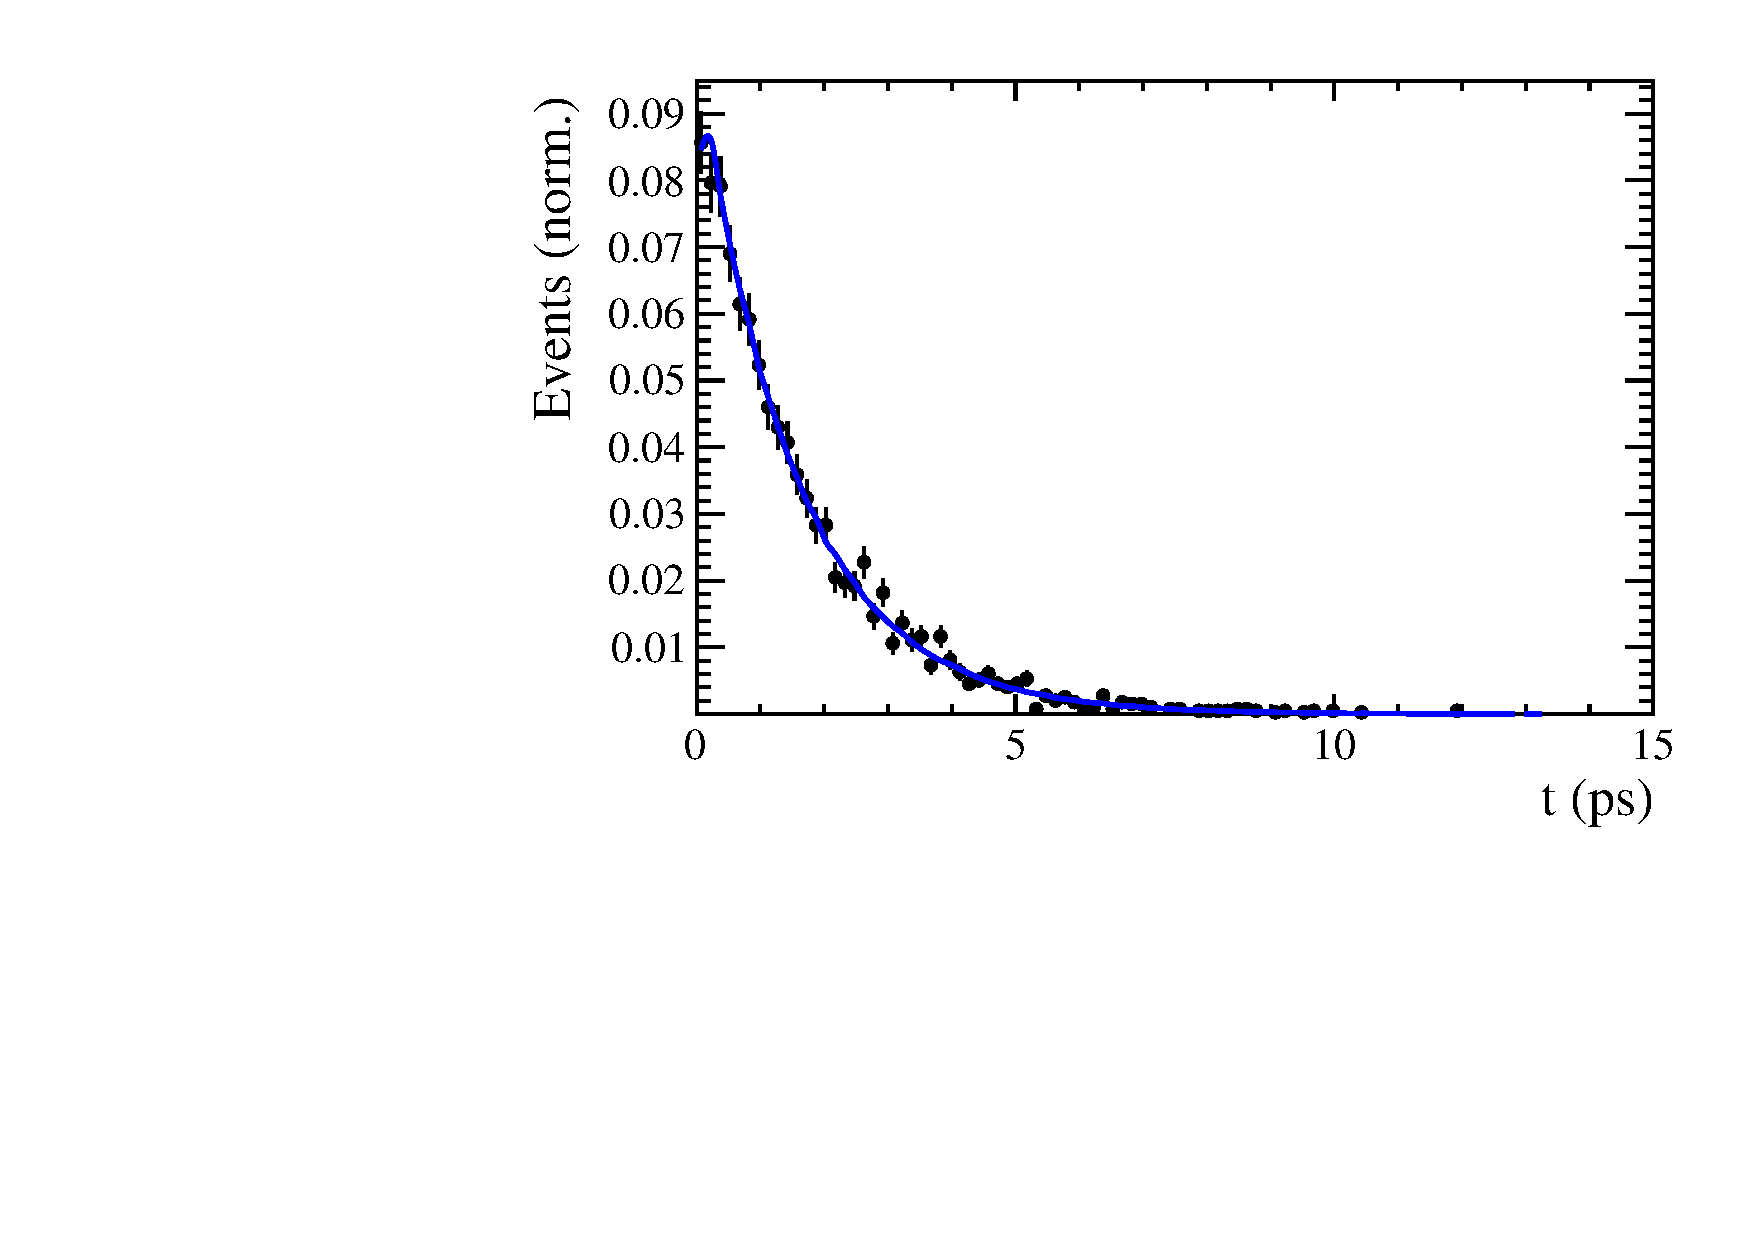
\includegraphics[width=0.45\textwidth, height = !]{figs/timeFit/signal_DsKpipi_CPV_MC/h_t.pdf} 
		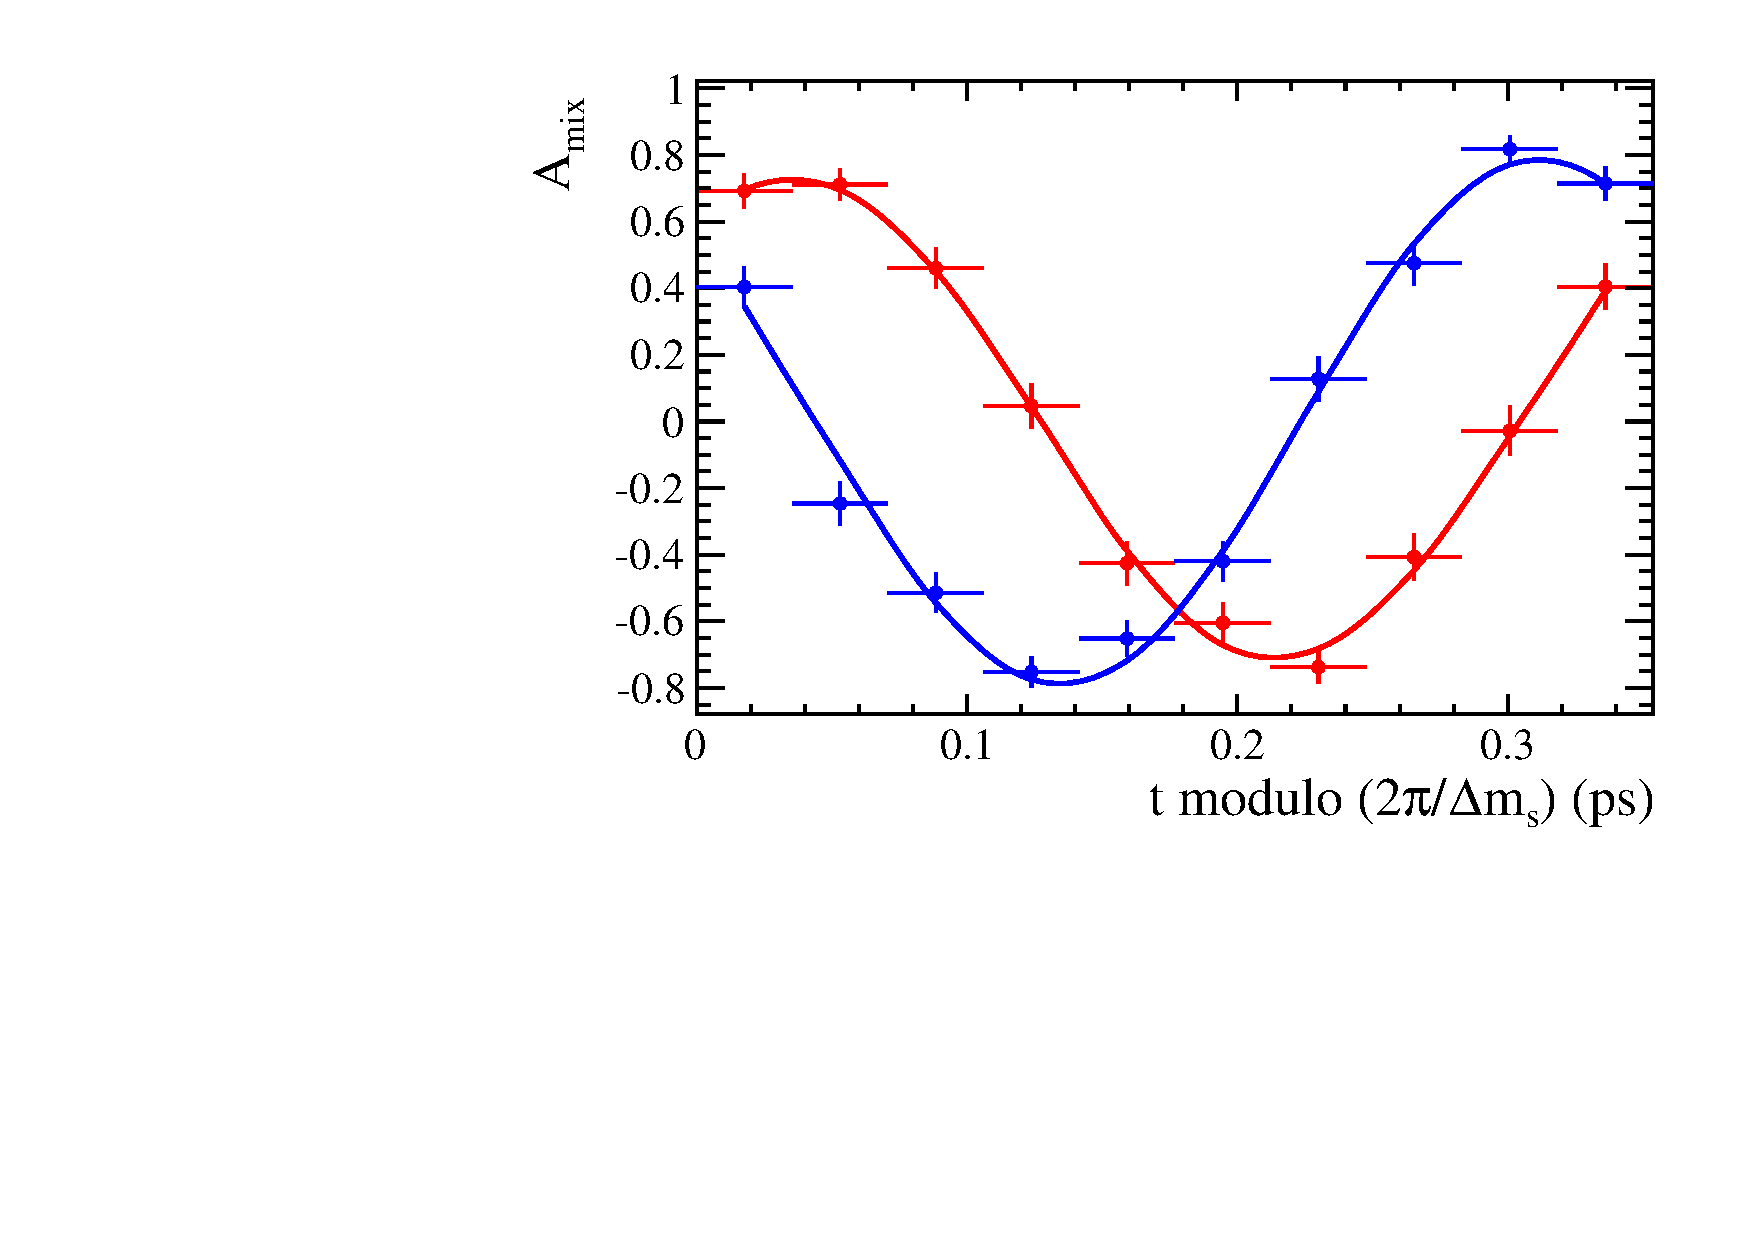
\includegraphics[width=0.45\textwidth, height = !]{figs/timeFit/signal_DsKpipi_CPV_MC/h_asym.pdf} 

		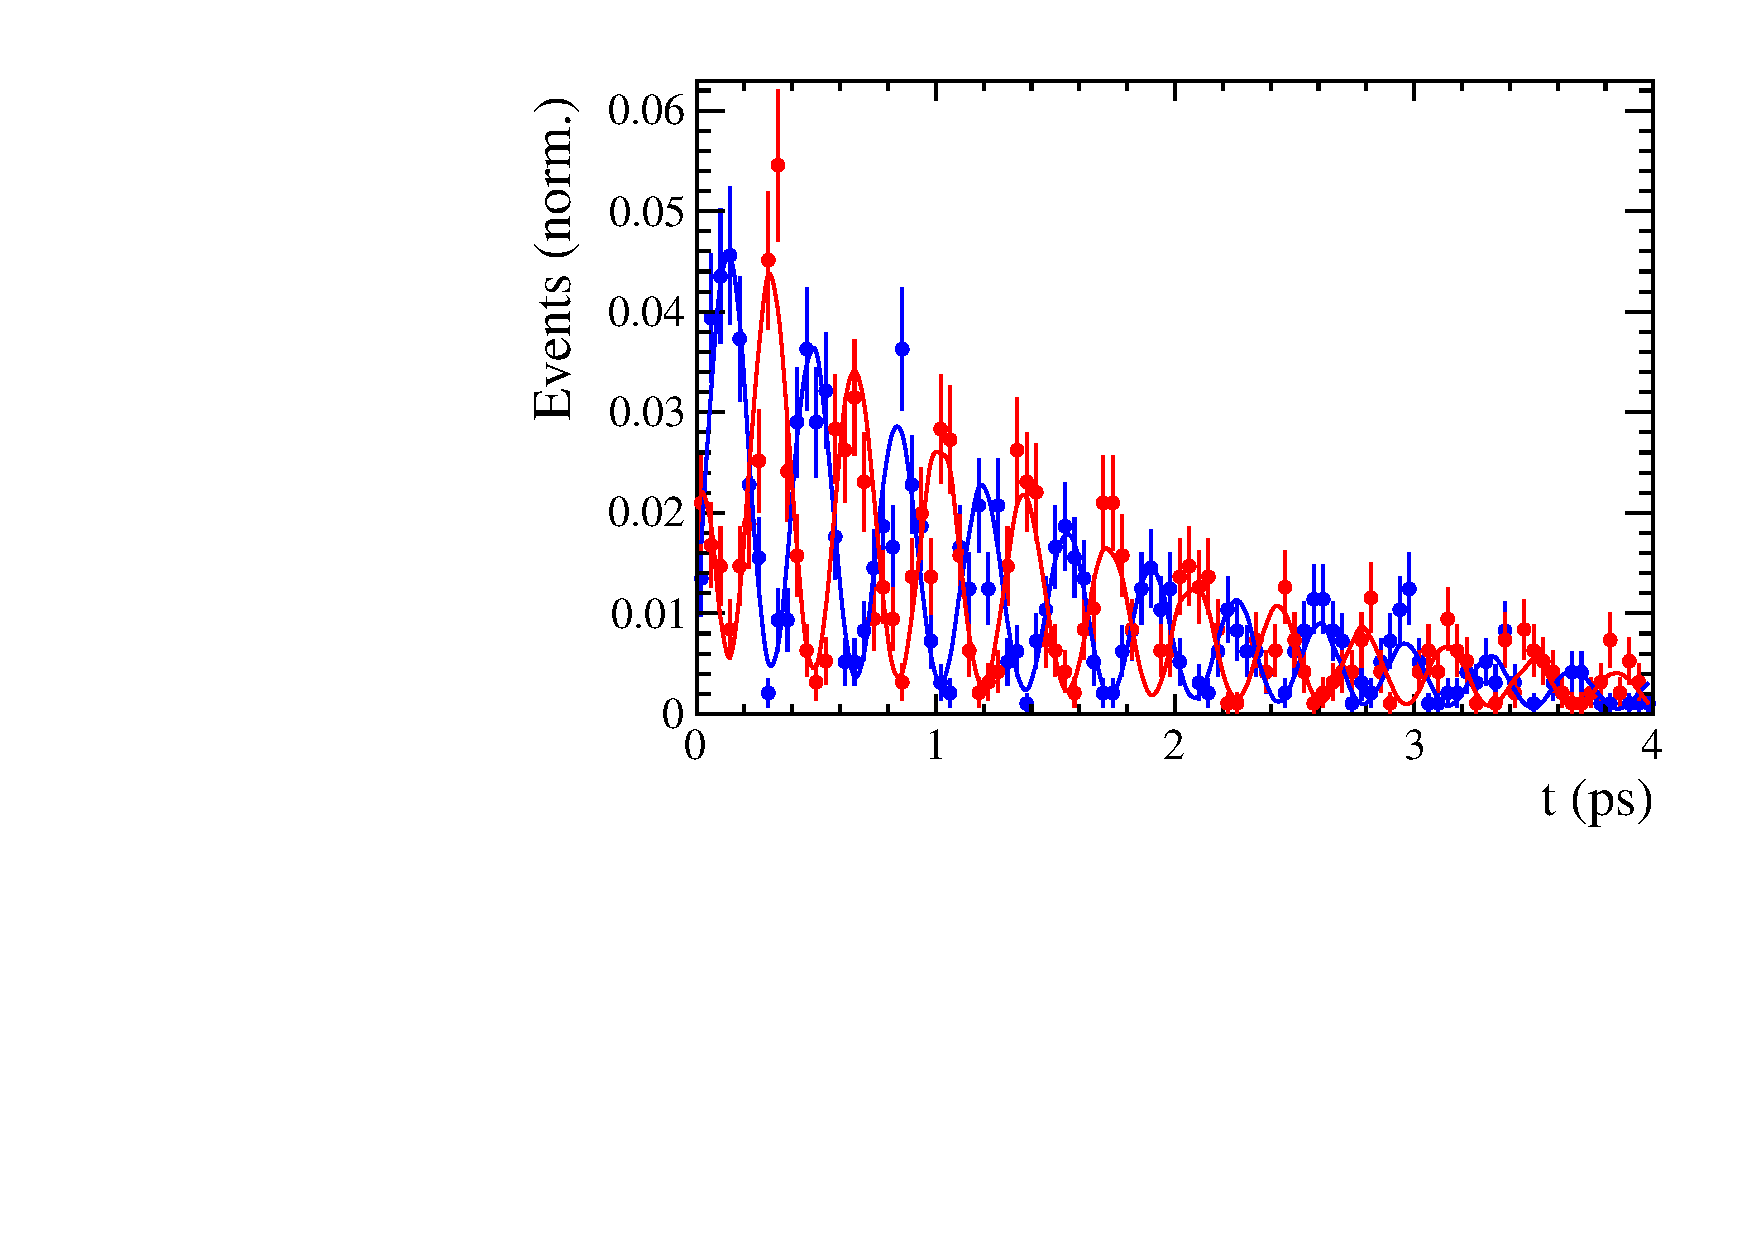
\includegraphics[width=0.45\textwidth, height = !]{figs/timeFit/signal_DsKpipi_CPV_MC/h_t_mixed_m.pdf} 
		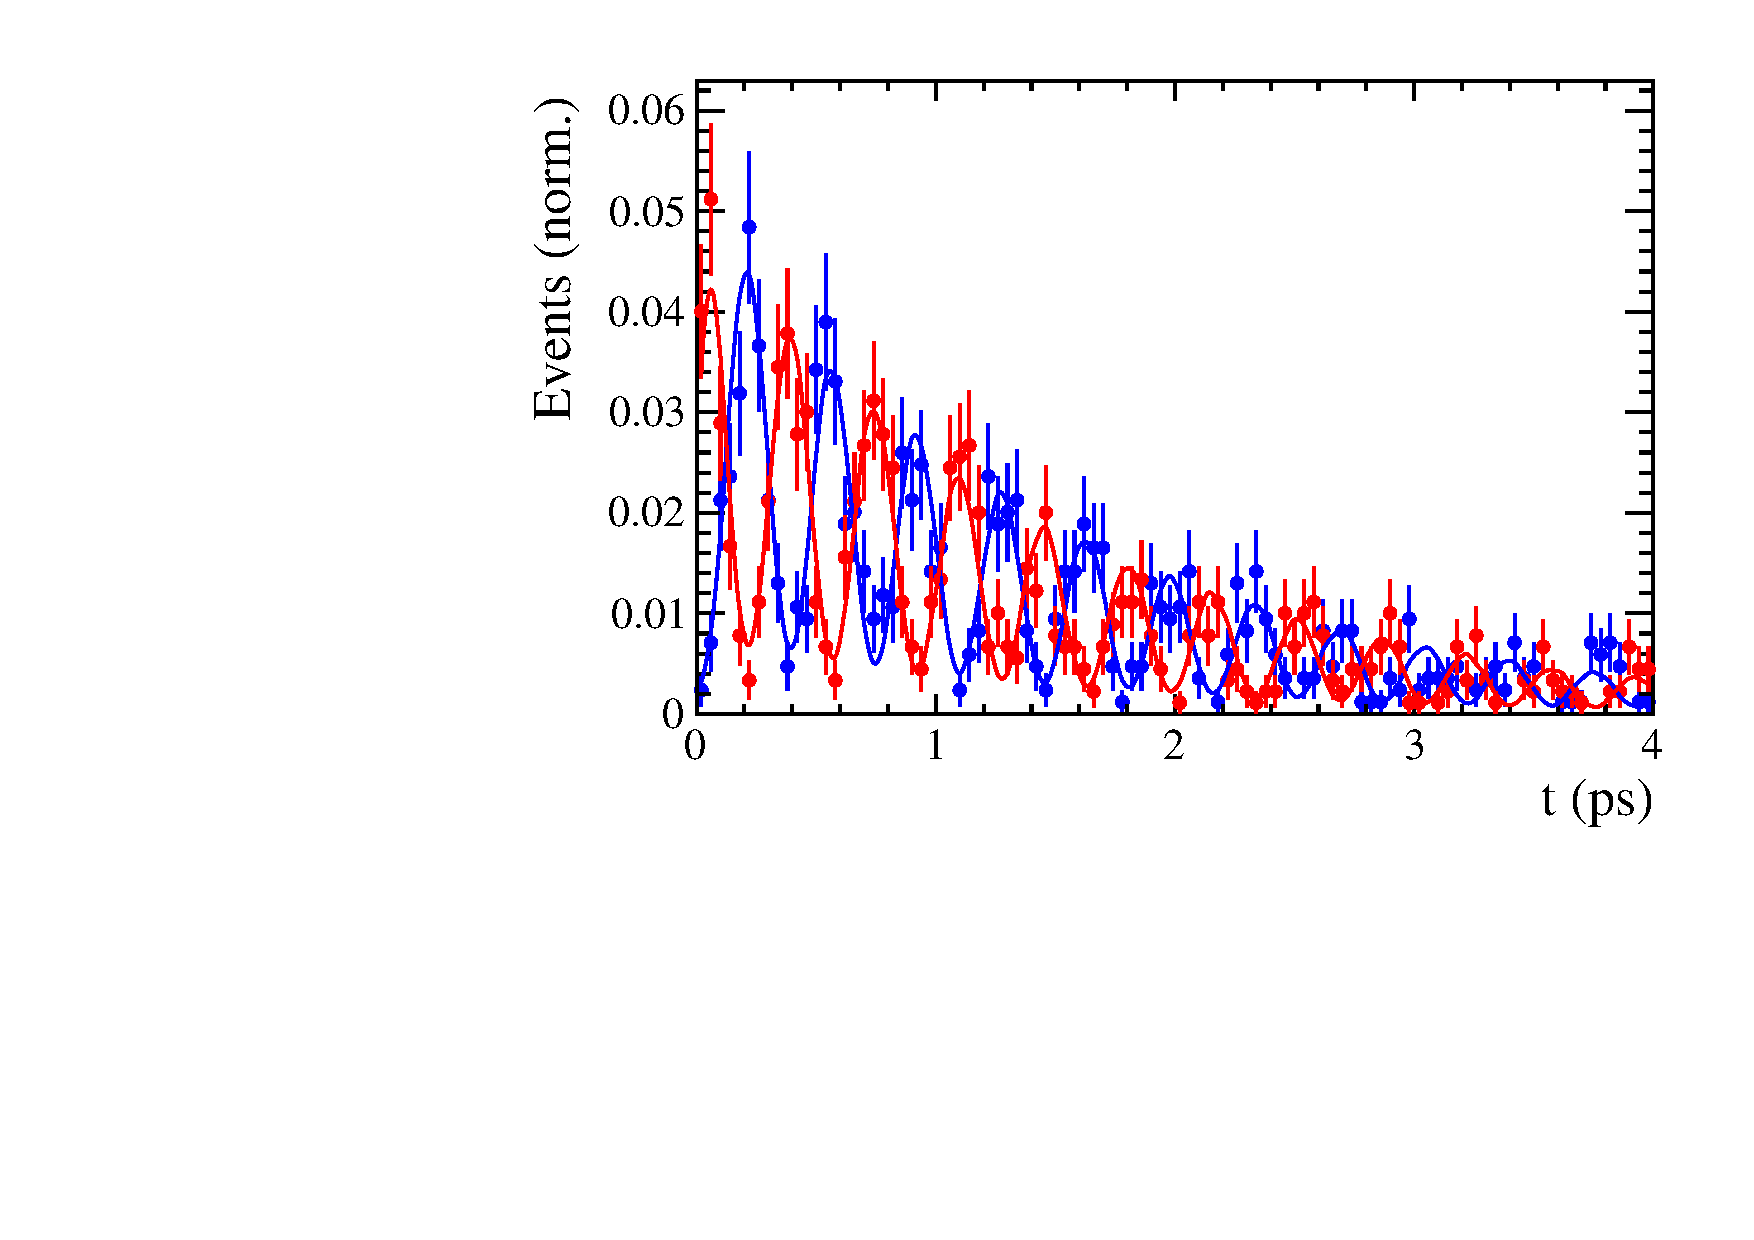
\includegraphics[width=0.45\textwidth, height = !]{figs/timeFit/signal_DsKpipi_CPV_MC/h_t_mixed_p.pdf} 
		
		\caption{Time distribution of $B_s \to D_s K \pi\pi$ events generated with \textsf{EVTGEN} (points with error bars) and \textsf{MINT2} fit projections (blue solid line).} 		
\end{figure}	

\begin{figure}[h]
	\centering
		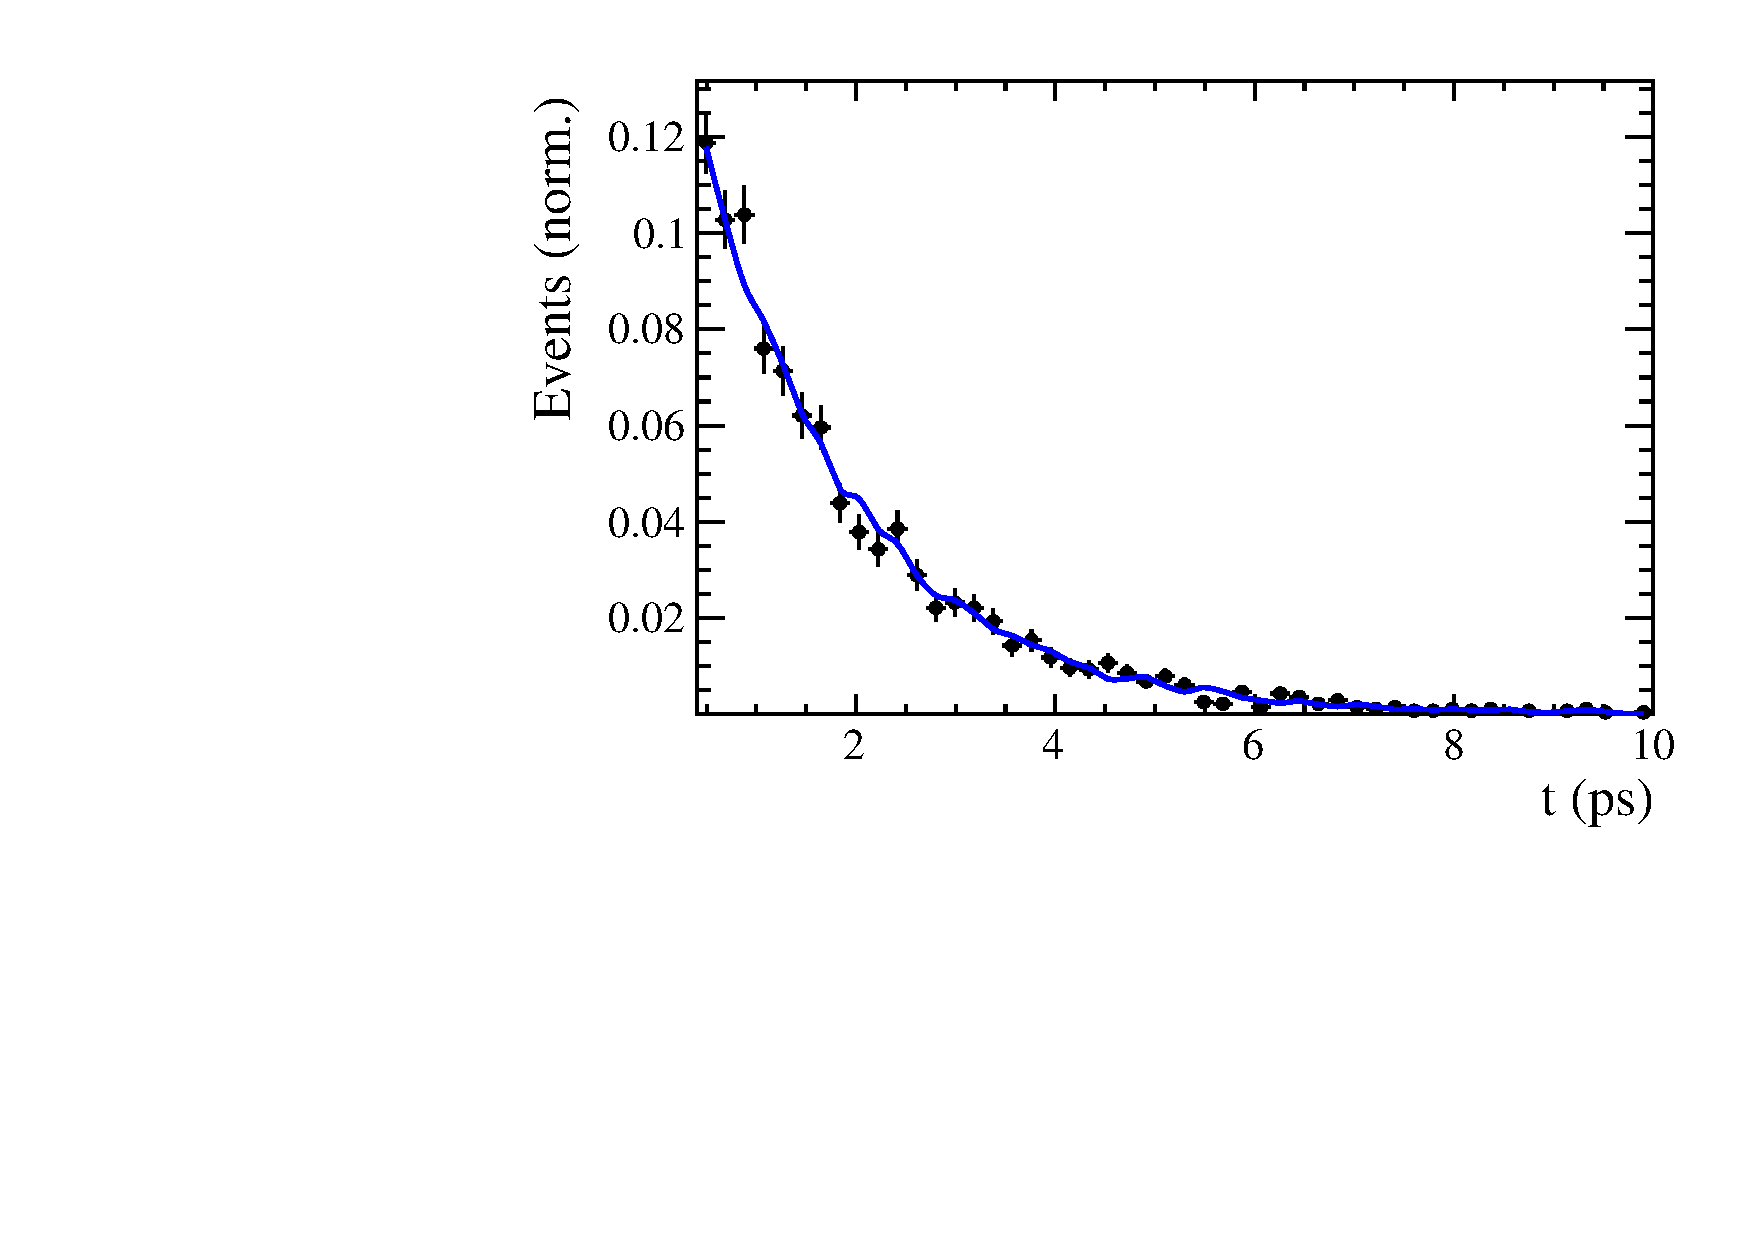
\includegraphics[width=0.3\textwidth, height = !]{figs/fullFit/signal_DsKpipi_CPV_MC/h_t.pdf} 
		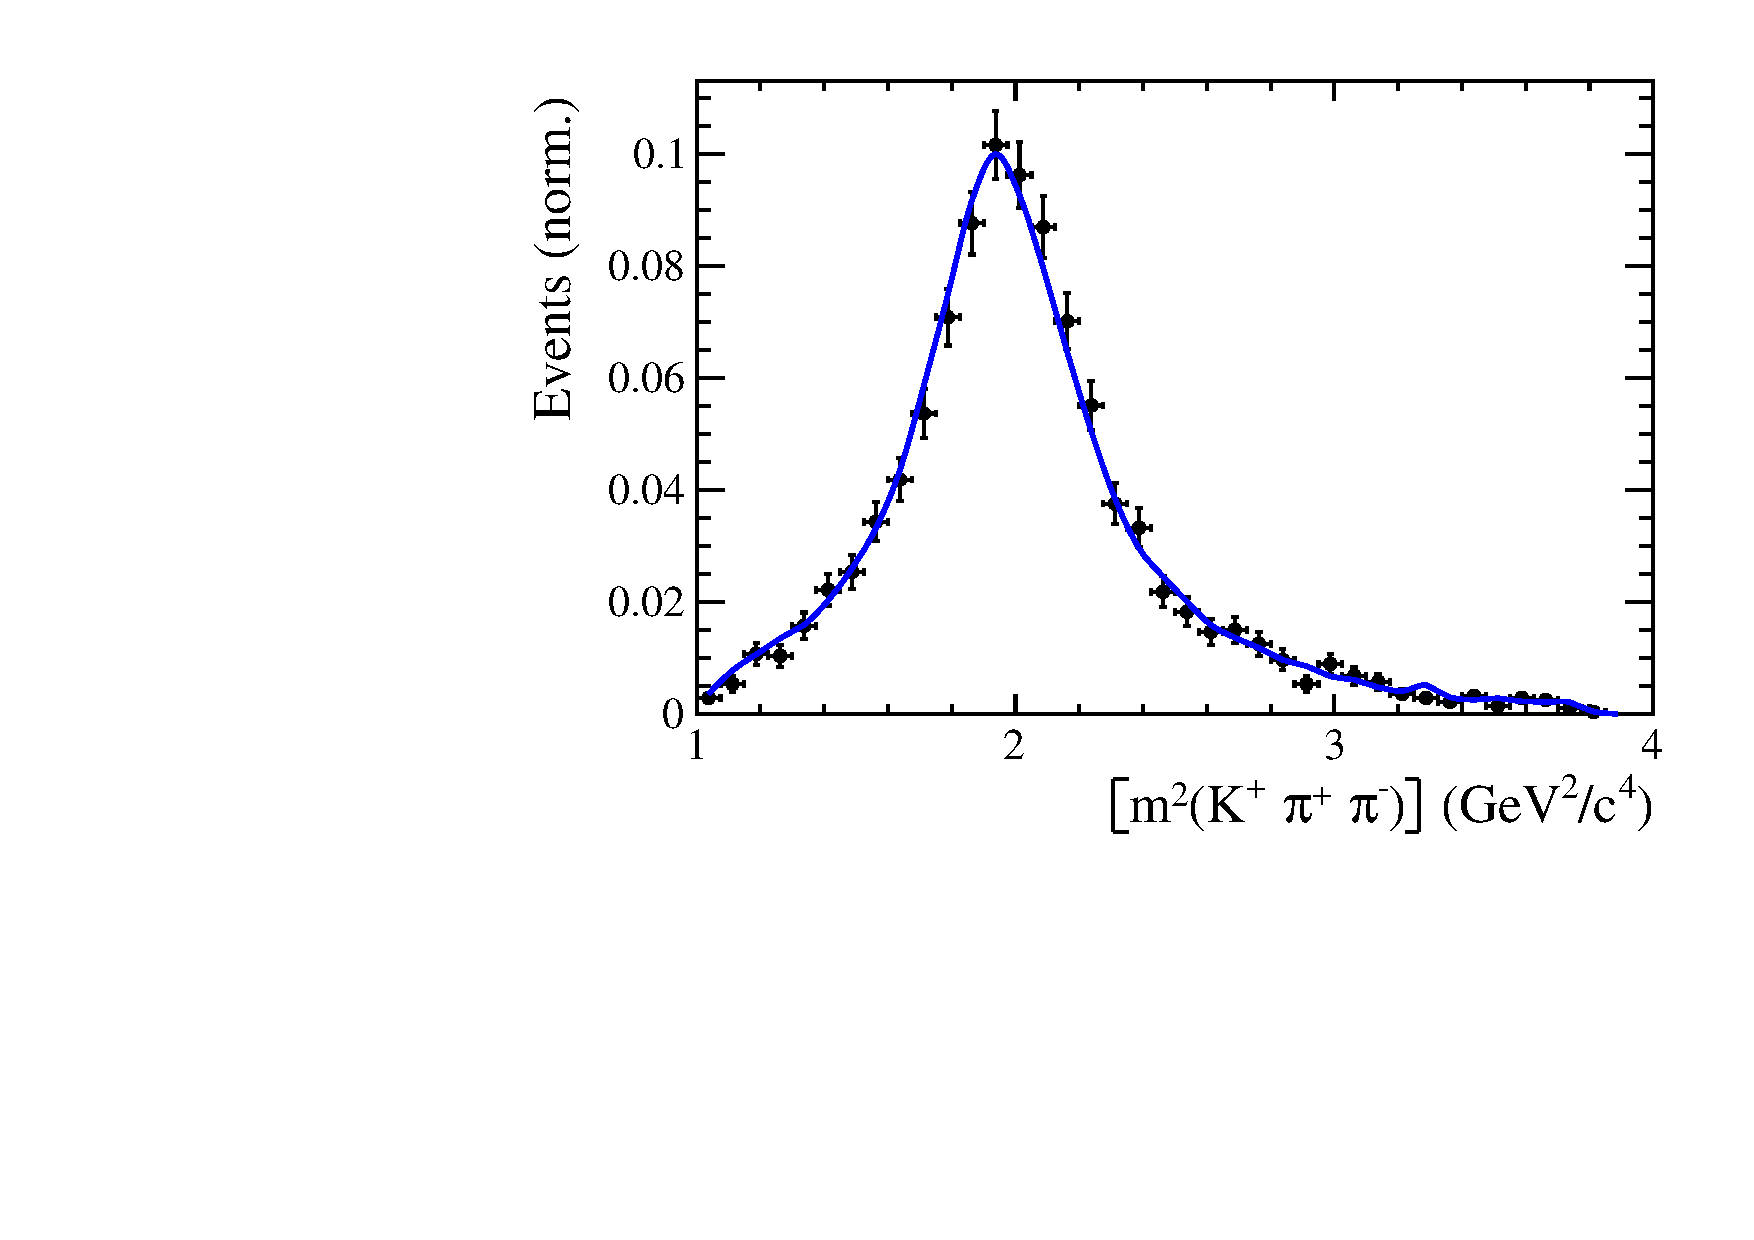
\includegraphics[width=0.3\textwidth, height = !]{figs/fullFit/signal_DsKpipi_CPV_MC/s_Kpipi.pdf} 
		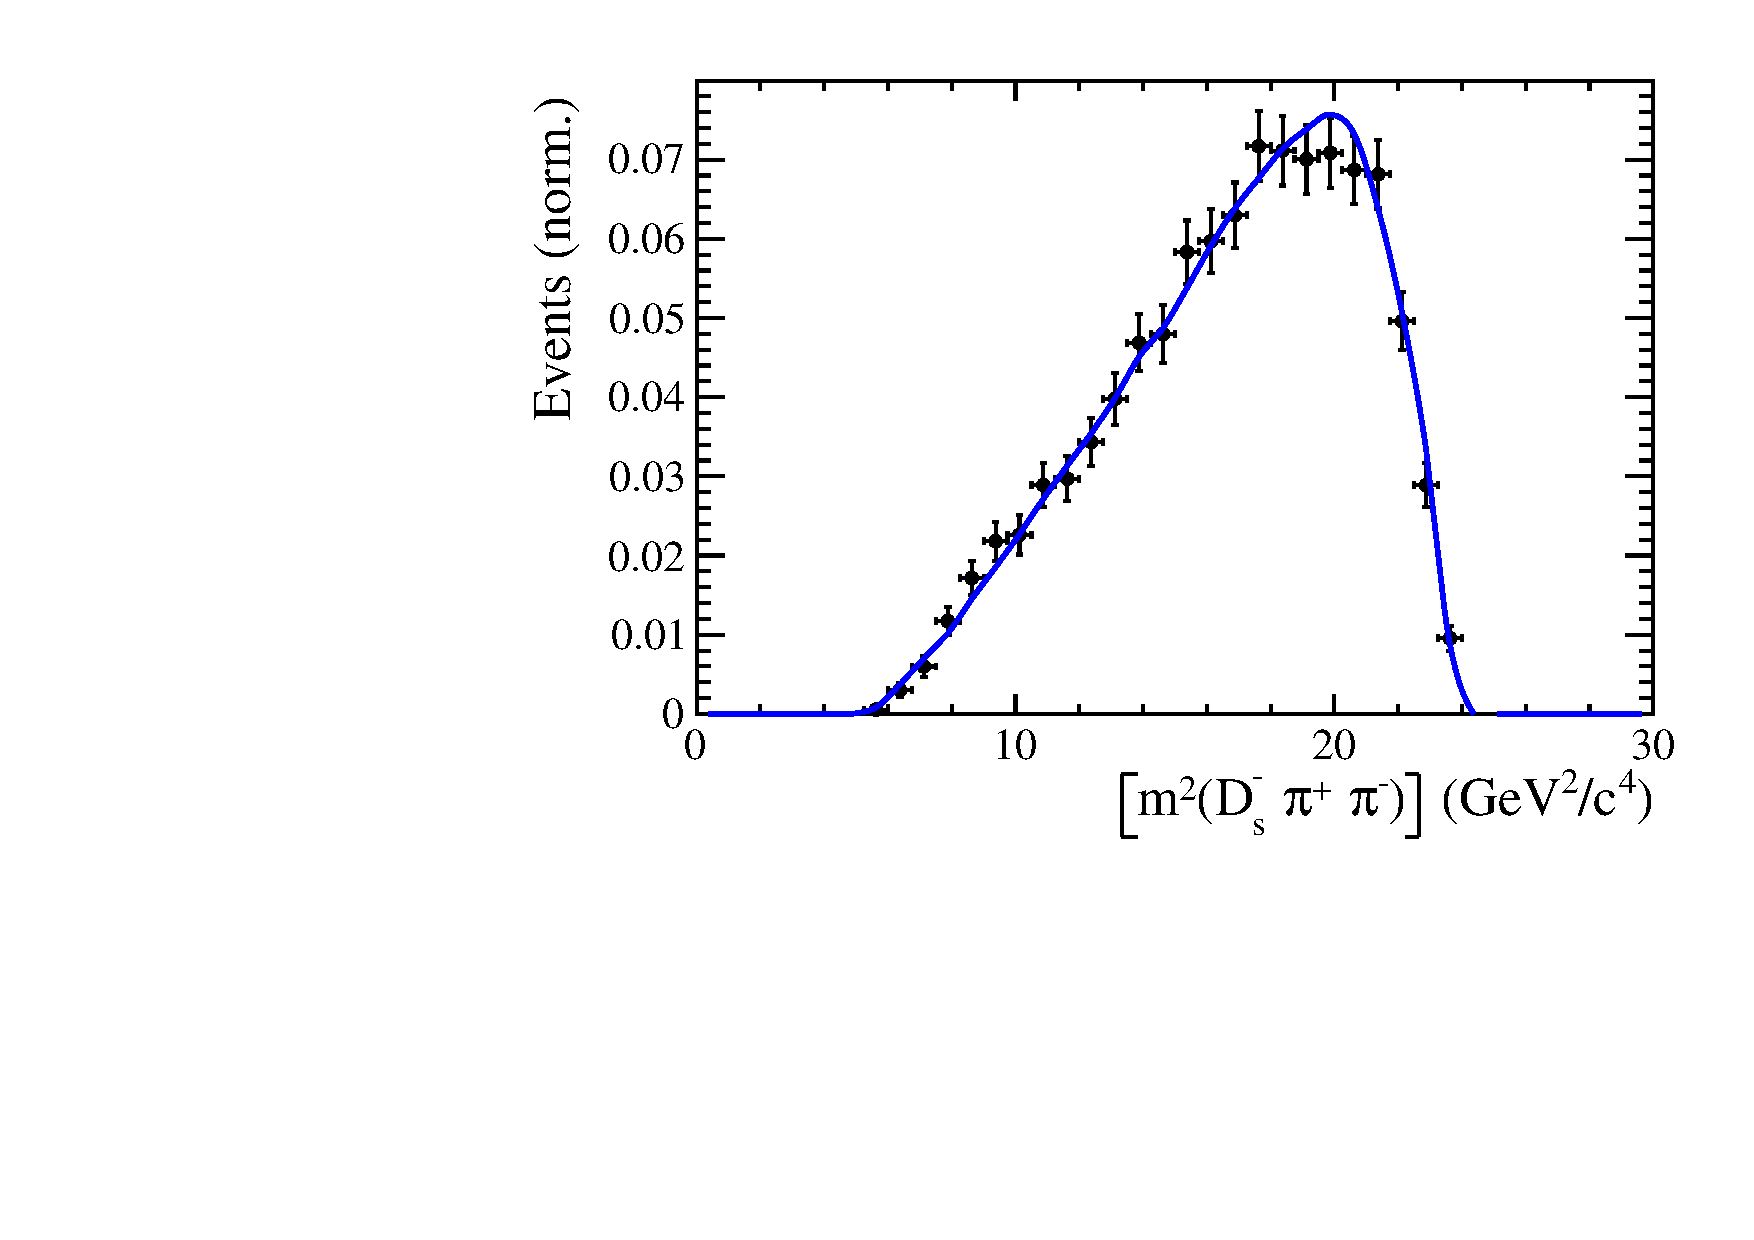
\includegraphics[width=0.3\textwidth, height = !]{figs/fullFit/signal_DsKpipi_CPV_MC/s_Dspipi.pdf} 

		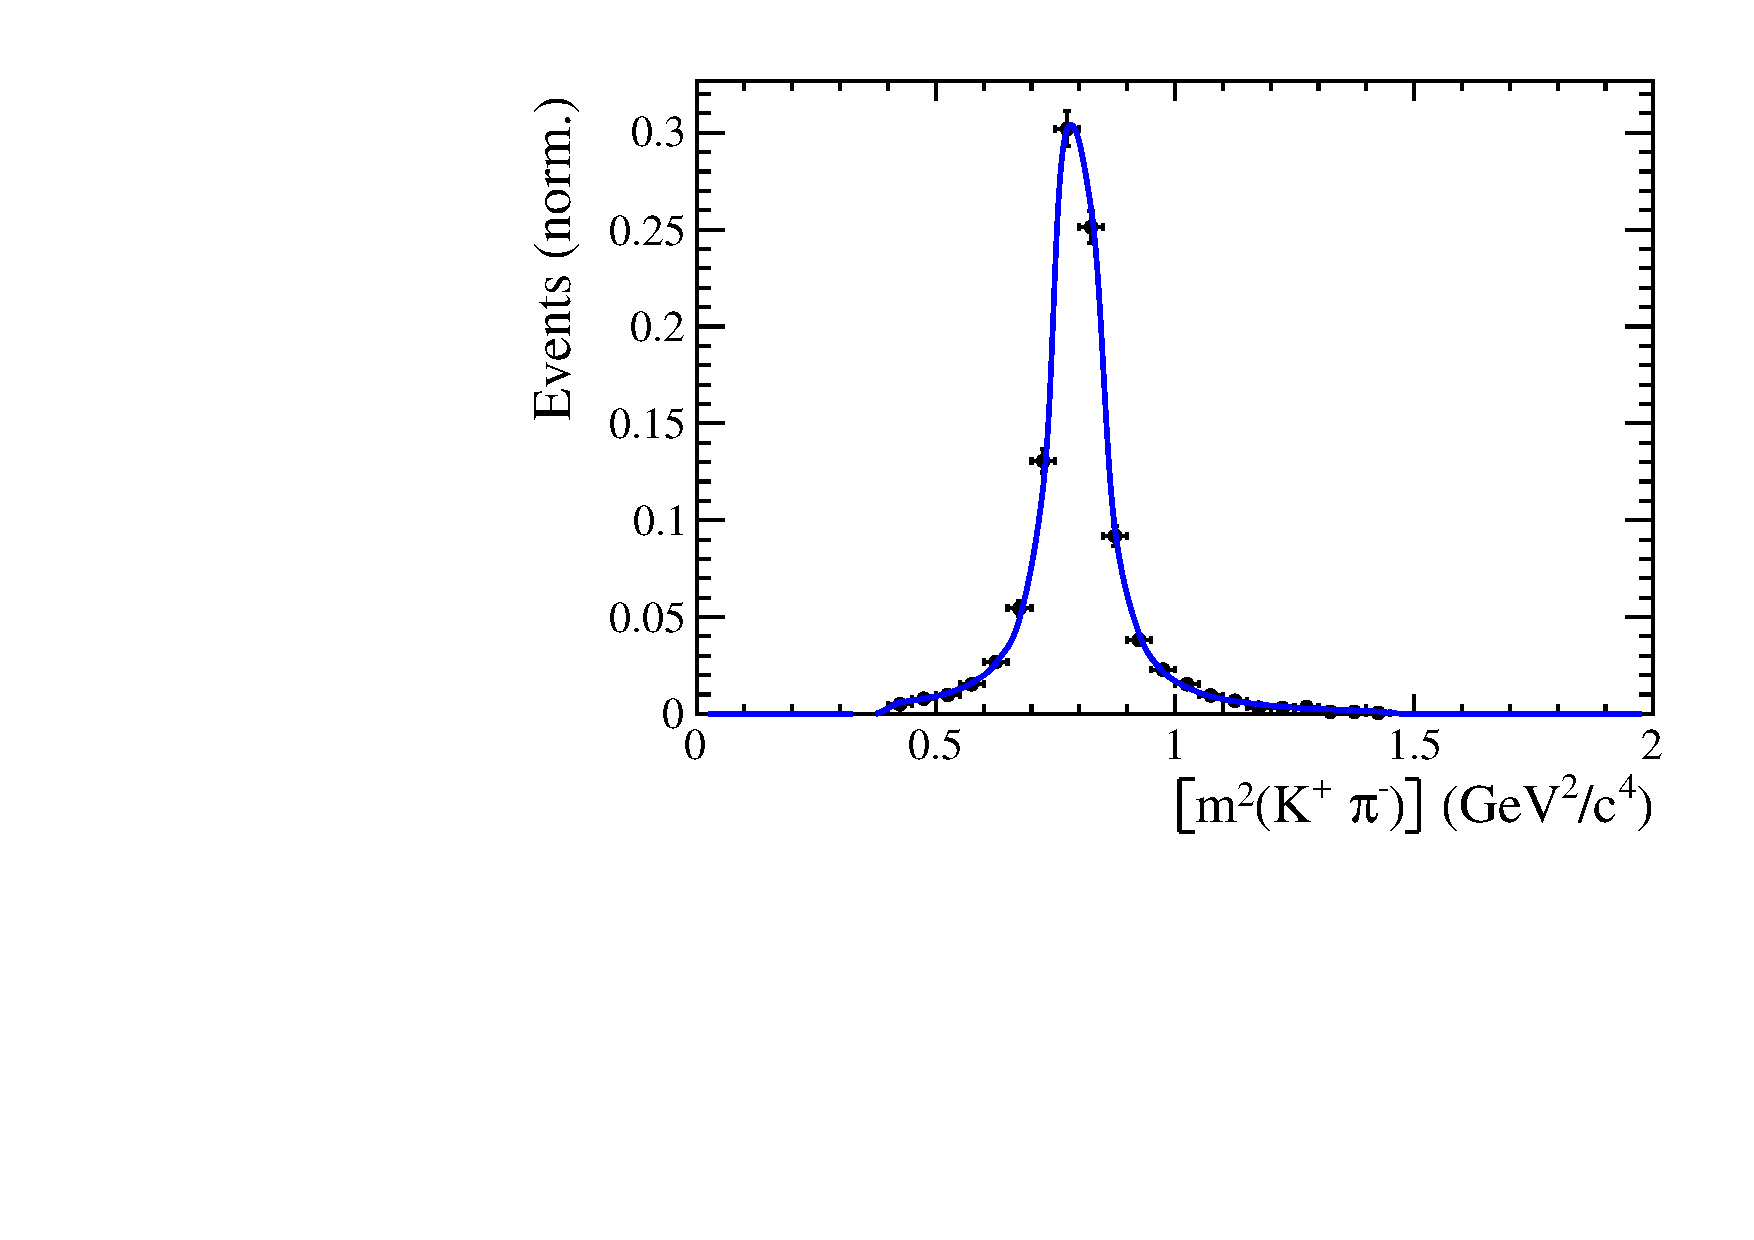
\includegraphics[width=0.3\textwidth, height = !]{figs/fullFit/signal_DsKpipi_CPV_MC/s_Kpi.pdf} 
		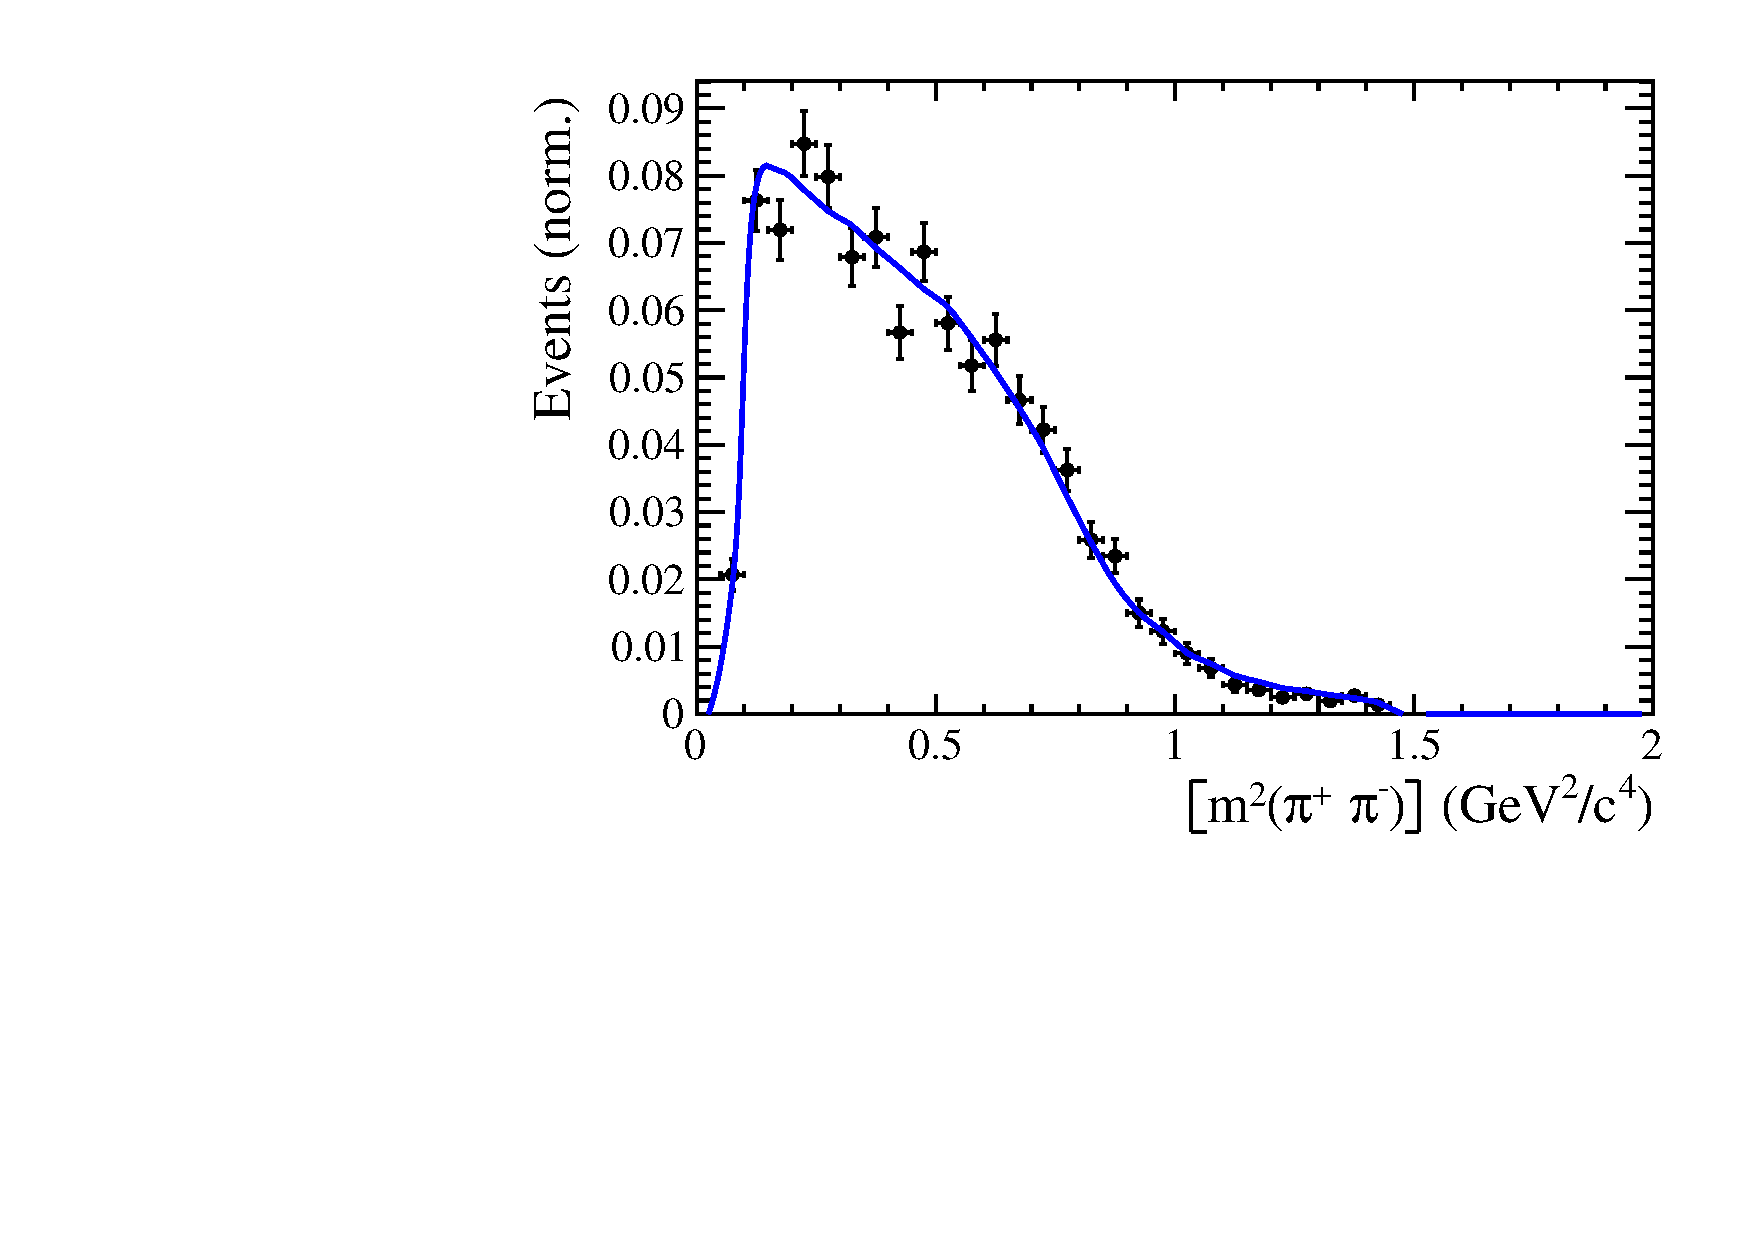
\includegraphics[width=0.3\textwidth, height = !]{figs/fullFit/signal_DsKpipi_CPV_MC/s_pipi.pdf} 
		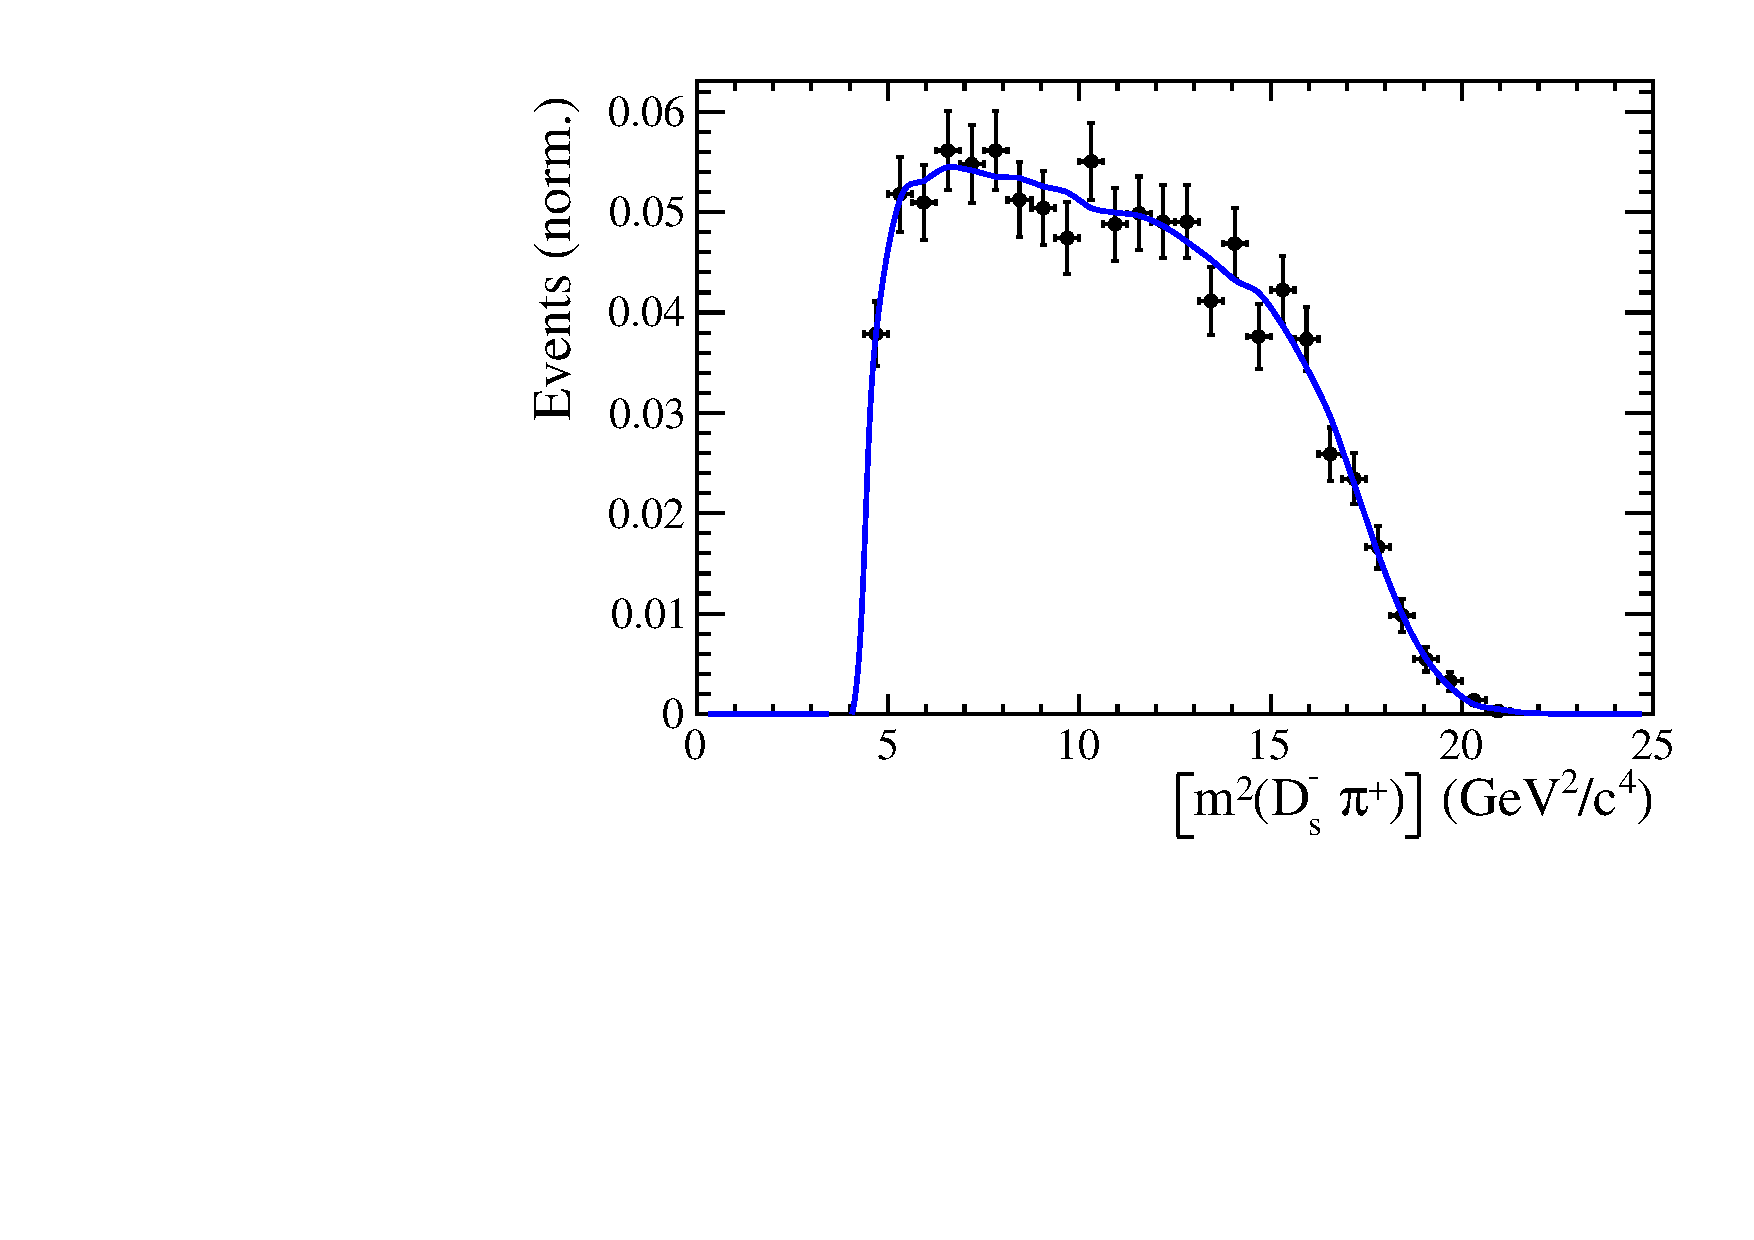
\includegraphics[width=0.3\textwidth, height = !]{figs/fullFit/signal_DsKpipi_CPV_MC/s_Dspi.pdf} 
		
		\caption{Time and invariant mass distributions of $B_s \to D_s K \pi\pi$ events generated with \textsf{EVTGEN} (points with error bars) and \textsf{MINT2} fit projections (blue solid line).} 		
\end{figure}	

\begin{table}[h]
\caption{Result of the phasespace-integrated fit to \textsf{EVTGEN} toy events.} 		
%  \scriptsize
  \centering
  \begin{tabular}
    {l c c}
    \hline \hline
    & Generated &  Fit result  \\   \hline
    $C$ &   &  	 \\
    $D$ &   &  	 \\
    $\bar D$ &   &  	 \\
    $S$ &   &  	 \\
    $\bar S$ &   &  	 \\
    \hline \hline
  \end{tabular}
    \label{tab:FitGenMC}
\end{table}

\begin{table}[h]
\caption{Result of the time-dependent amplitude fit to \textsf{EVTGEN} toy events.} 		
%  \scriptsize
  \centering
  \begin{tabular}
    {l c c}
    \hline \hline
    & Generated &  Fit result  \\   \hline
    $x_-$ &   &  	 \\
    $y_-$ &   &  	 \\
    $x_+$ &   &  	 \\
    $y_+$ &   &  	 \\
    \hline \hline
  \end{tabular}
    \label{tab:FitGenMC2}
\end{table}

%\begin{table}[h]
%\caption{} 		
%%  \scriptsize
%  \centering
%  \begin{tabular}
%    {l c c c c}
%    \hline \hline
%    & Generated &  Full PDF     &   Phasespace integrated  \\   \hline
%	$r$ & 0.4 & $0.38 \pm 0.06$   &  unstable \\
%	$\kappa$  & \textcolor{red}{0.2} & $0.23 \pm 0.13$ & 0.2 (fixed)  \\
%	$\delta$ & 100 & $99 \pm 22$ &  unstable\\
%	$\gamma$ & 70 & $70 \pm 17$  & unstable \\
%    \hline \hline
%  \end{tabular}
%\end{table}


%\subsection{Estimation of coherence factor}
%
%To estimate the coherence factor we could generate many toys with random $a_i$ and $\bar a_i$ values (see https://twiki.cern.ch/twiki/pub/LHCbPhysics/Bu2DKstar/LHCb-ANA-2017-005\_v1.pdf) using the set of amplitudes show in our last talk. However with so many interfering amplitudes, I would be surprised if you couldn't generate every possible value for $\kappa$. In any case, this would give us a  range where to expect possible values for $\kappa$. Worst case would be $0 \leq \kappa \leq 1$. \\
%
%Assumptions:
%	\begin{itemize}
%		\item   $A(x) = \sum_i a_i \, A_i(x)$   \\
%		 $\bar A(x) = \sum_i \bar a_i \, \bar A_i(x)$
%		\item Use amplitudes from flavor-averaged, time-integrated fit
%		 \item Draw random $a_i$ and $\bar a_i $ values
%		 \item Constraints: \\
%		 $\int ( \vert a_i  A_i(x) \vert^2 + \vert \bar a_i  \bar A_i(x) \vert^2 ) \, \text{d}x / N = F^{eff}_i $ \\
%		 $r \approx 0.4 $ (ration of CKM elements)
%	\end{itemize}
%	
%\begin{figure}[hp]
%	\centering
%		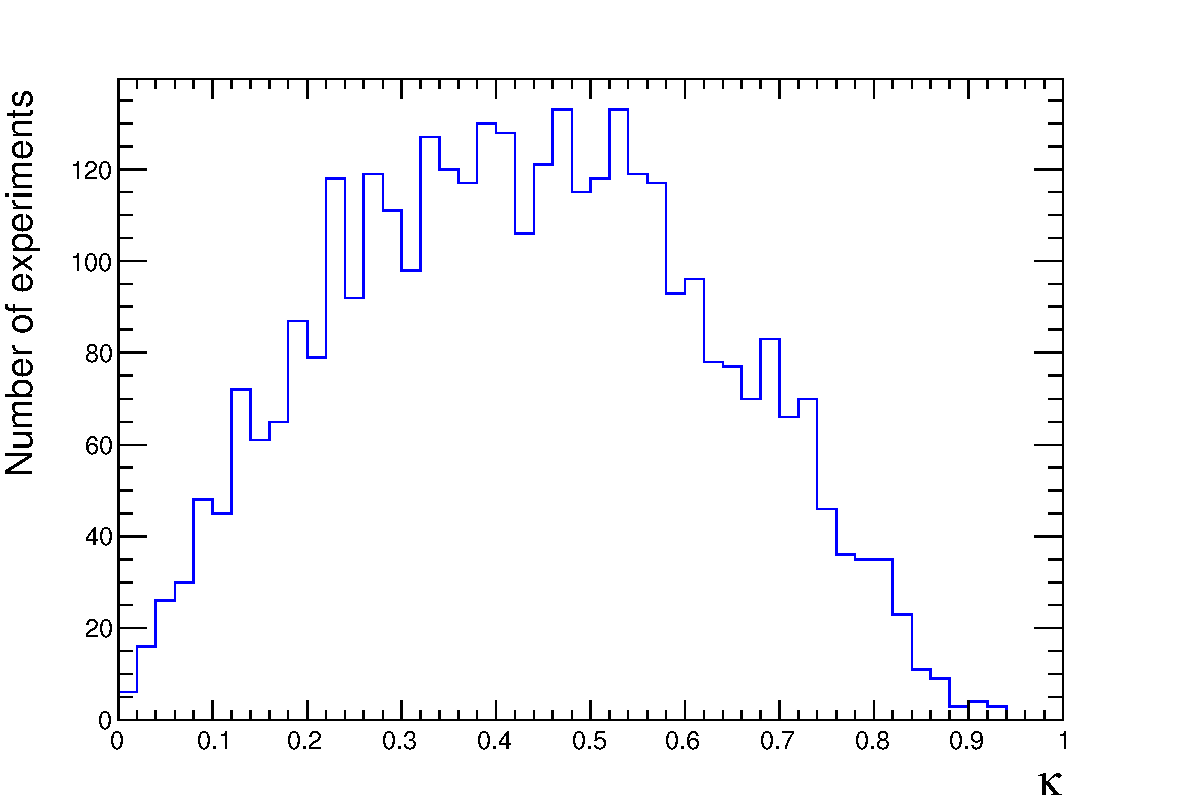
\includegraphics[width=0.35\textwidth, height = 3.cm]{figs/plots/k-eps-converted-to.pdf} 
%		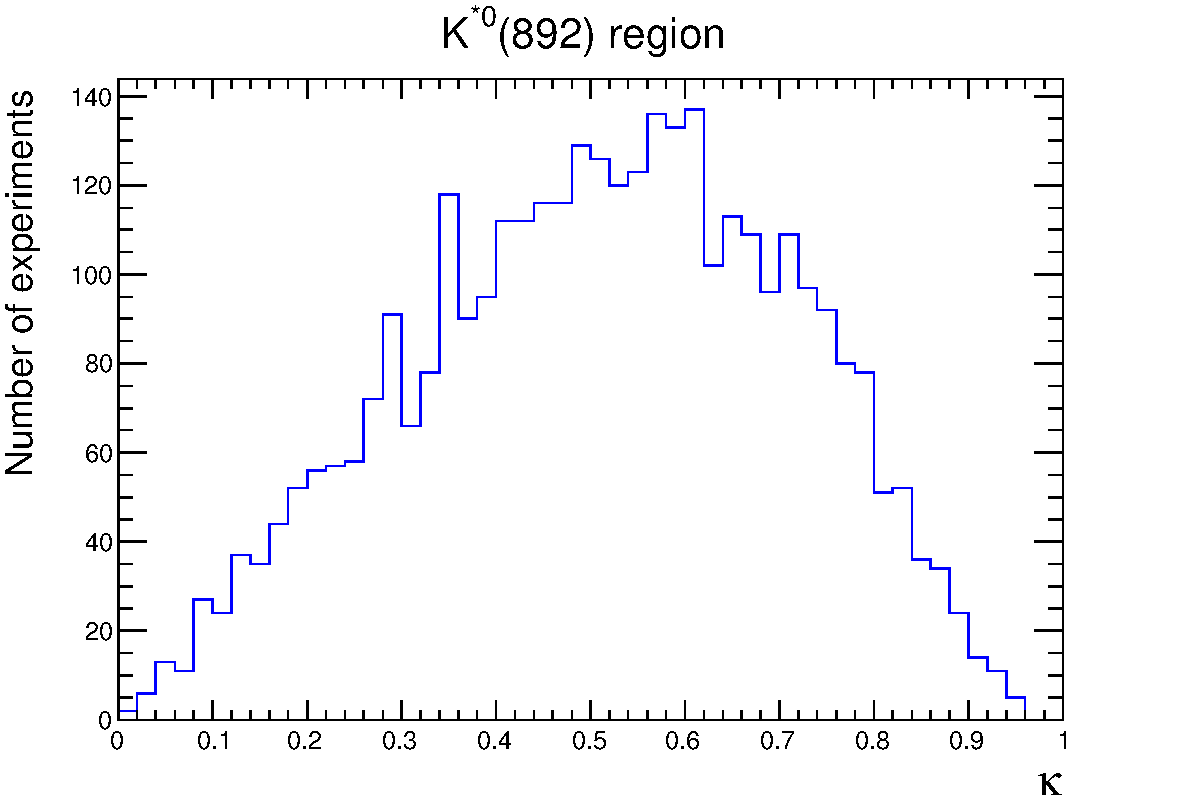
\includegraphics[width=0.35\textwidth, height = 3.cm]{figs/plots/k_Ks-eps-converted-to.pdf} 
%		
%		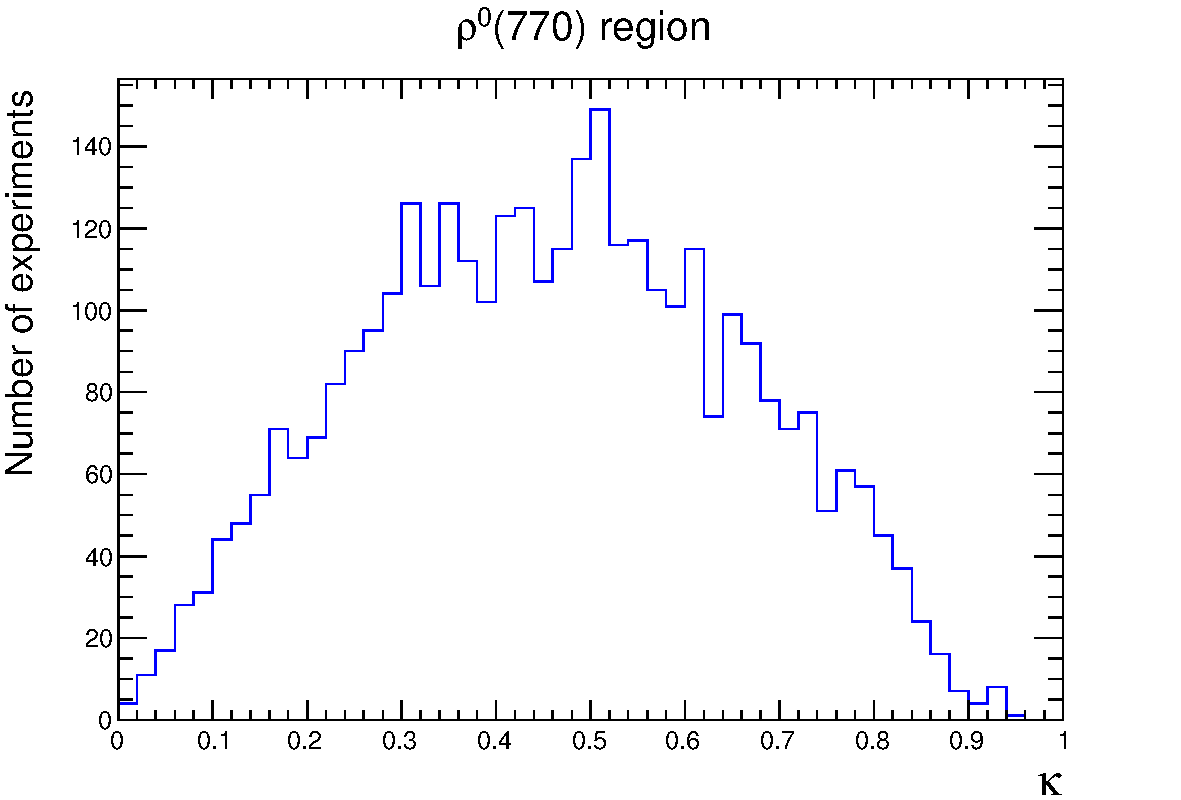
\includegraphics[width=0.35\textwidth, height = 3.cm]{figs/plots/k_rho-eps-converted-to.pdf} 
%		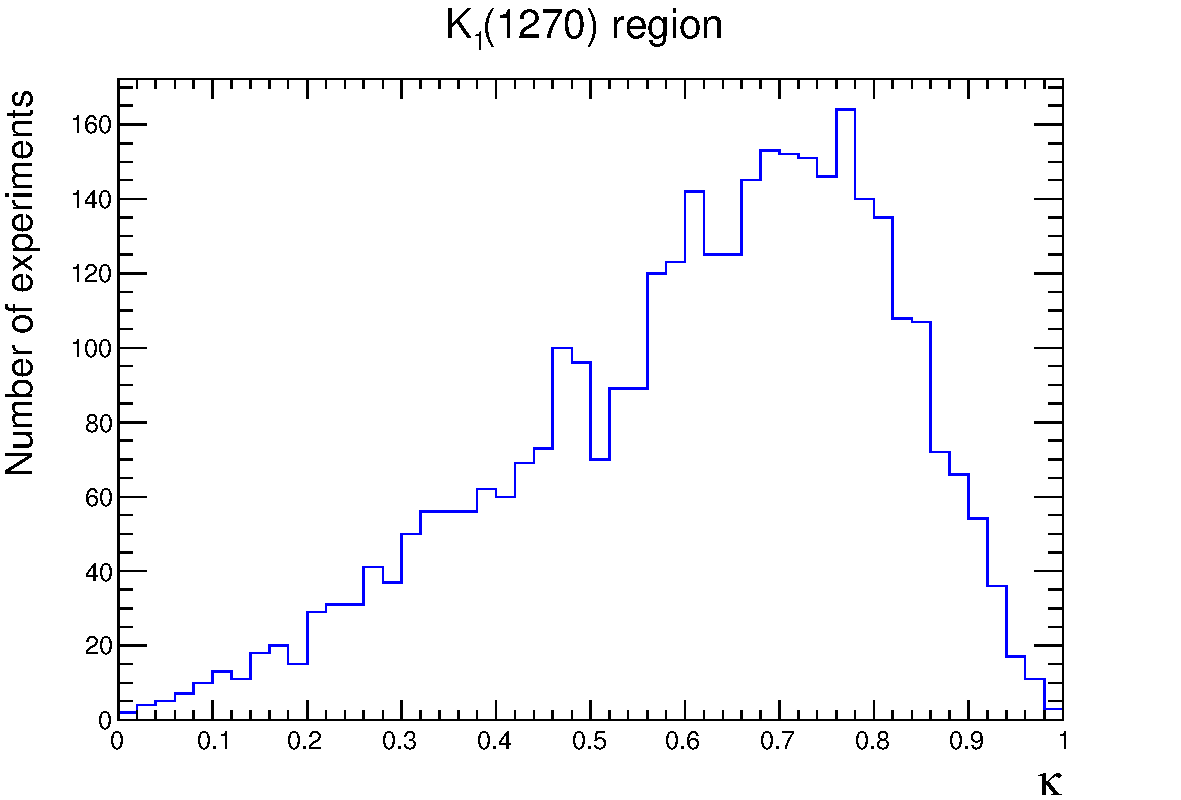
\includegraphics[width=0.35\textwidth, height = 3.cm]{figs/plots/k_K1-eps-converted-to.pdf} 	
%		\caption{}	
%\end{figure}		
%
%	\begin{table}[h]
%			\caption{}	
%  \footnotesize
%  \centering
%  \begin{tabular}
%    {l c c }
%    \hline \hline
%    Region &  $<\kappa> (\%)$   &  Cut eff. $(\%)$ \\   \hline
%    Full & 43 &  100 \\
%    $K^*(892)$ & 51    &  43  \\
%    $\rho^0(770)$ & 46  & 47   \\
%    $K_1(1270)$ & 61   & 23  \\
%    \hline \hline
%  \end{tabular}
%  \label{tab:sideband}
%\end{table}


%The next option would be to fit the flavor tagged Dalitz plot which would allow us to really predict $\kappa$ (together with $r$ and $\delta$ actually). 
%Integrating the full pdf over  time, we get
%\begin{align*}
%	\int P(x,t,q_t,q_f) \text d t &\propto   
%	 \left( \vert A(x) \vert^2 + \vert \bar A(x) \vert^2 \right) \, \frac{4\Gamma}{4\Gamma^2-\Delta \Gamma^2} \\
%	 & + q_t q_f \left( \vert A(x) \vert^2 - \vert \bar A(x) \vert^2 \right) \, \frac{\Gamma}{\Gamma^2+m_s^2} \\
%	 & -2 \text{Re}\left( A(x)^{*}  \bar A(x) \, e^{-i q_f (\gamma - 2\beta_s)}  \right) \,\frac{2\Delta\Gamma}{4\Gamma^2-\Delta \Gamma^2} \\
%	 & -2 q_t q_f \text{Im}\left( A(x)^{*}  \bar A(x) \, e^{-i q_f (\gamma - 2\beta_s)}  \right)\, \frac{m_s}{\Gamma^2+m_s^2} 
%\end{align*}
%
%I think that is a very interesting result since it shows that we could in principle also measure $\gamma$ with a time-independent 
%amplitude fit. But no idea how sensitive this would be. Probably not so much since the prefactors of the third and forth term are at least one order of 
%magnitude smaller than the first term.
%Unfortunately, the sensitivity to the coherence factor also comes mainly from the third and forth term. \\
%If we just want to estimate $\kappa$ from this fit and then use it for the lifetime fit, the potential $\gamma$ sensitivity of the Dalitz fit is another problem. 
%We could fix $\gamma$ to the world average for the dalitz fit but this might introduce some bias.
%Better would be to average over the final state flavor in which case the sensitivity to gamma would be lost. \\
%
%In summary, I think it is very hard to disentangle $A(x)$ and $\bar A(x)$ from a time integrated fit since the oscillation frequency is so large.
%We might be able to get some estimate but in the end, the lifetime fit has to determine the precise value.
%A full time dependent amplitude fit would of course be the most sensitive approach (but model-dependent).

%\clearpage
%\subsection{Sensitivity study}
%
%Assumptions:
%	\begin{itemize}	
%		\item Use amplitudes from flavor-averaged, time-integrated fit
%		\item $r = 0.4$ (ratio of CKM elements) 
%		\item PDG values for: $\tau,\Delta m_s, \Delta \Gamma, \beta_s$
%		\item $\epsilon(x,t) = const.$, perfect resolution  
%		\item $\epsilon_{Tag} = 0.66, <\omega> = 0.4 $   
%		\item $N_{signal} = 3000$ (Run1+15/16 data)		 
%	\end{itemize}
%	
%	
%		\begin{figure}[hp]
%	\centering
%		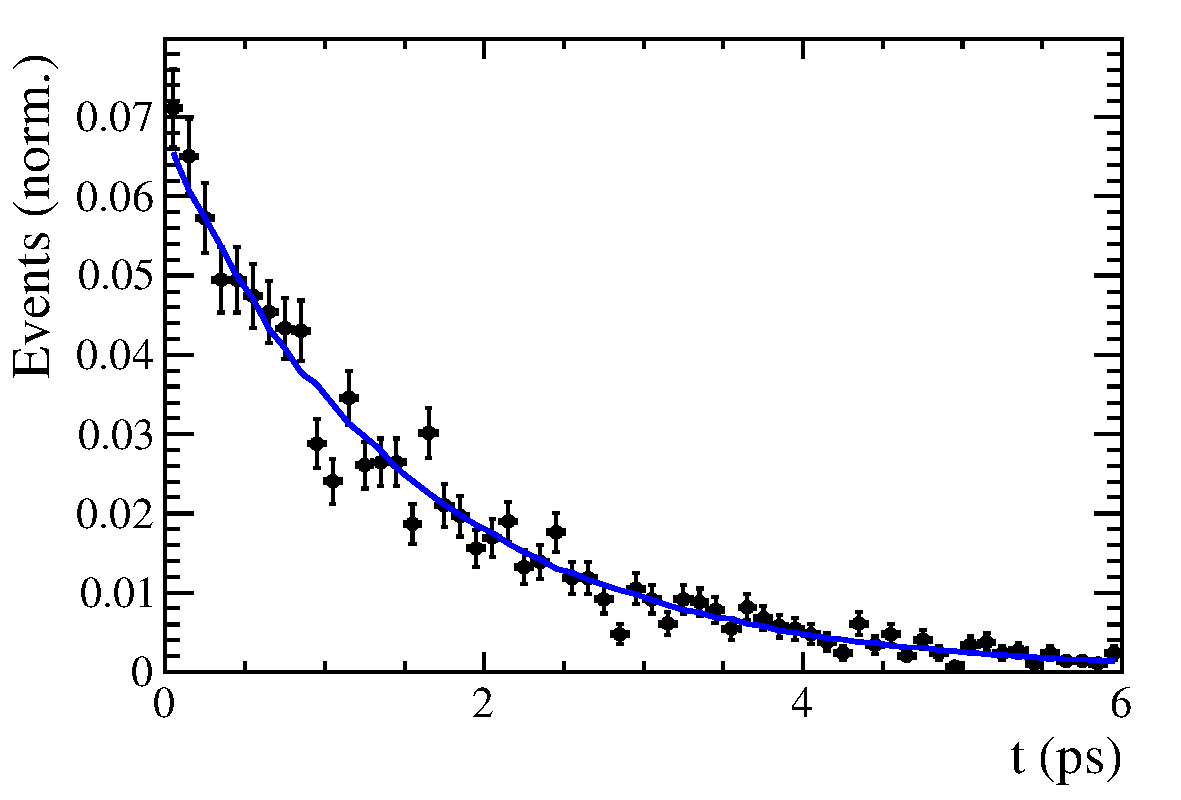
\includegraphics[width=0.45\textwidth, height = !]{figs/plots_toy/h_t-eps-converted-to.pdf} 
%		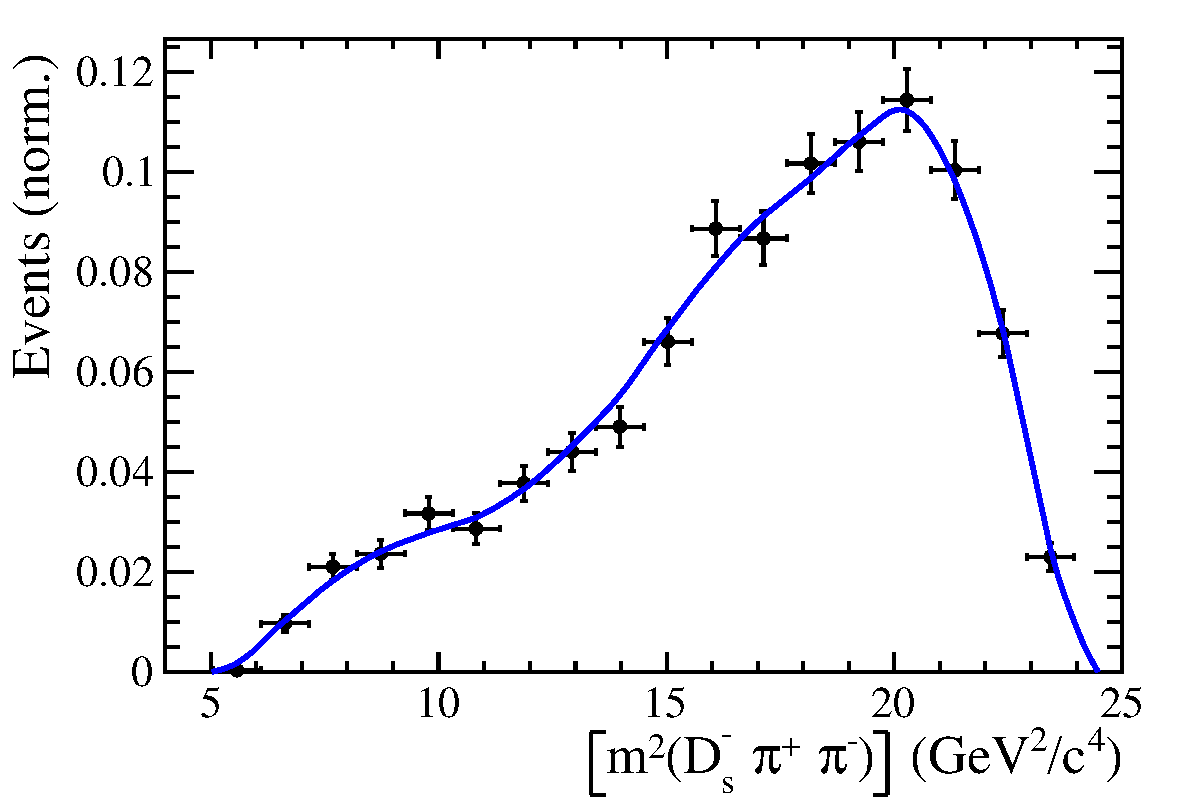
\includegraphics[width=0.45\textwidth, height = !]{figs/plots_toy/s_Dspipi-eps-converted-to.pdf} 
%		
%		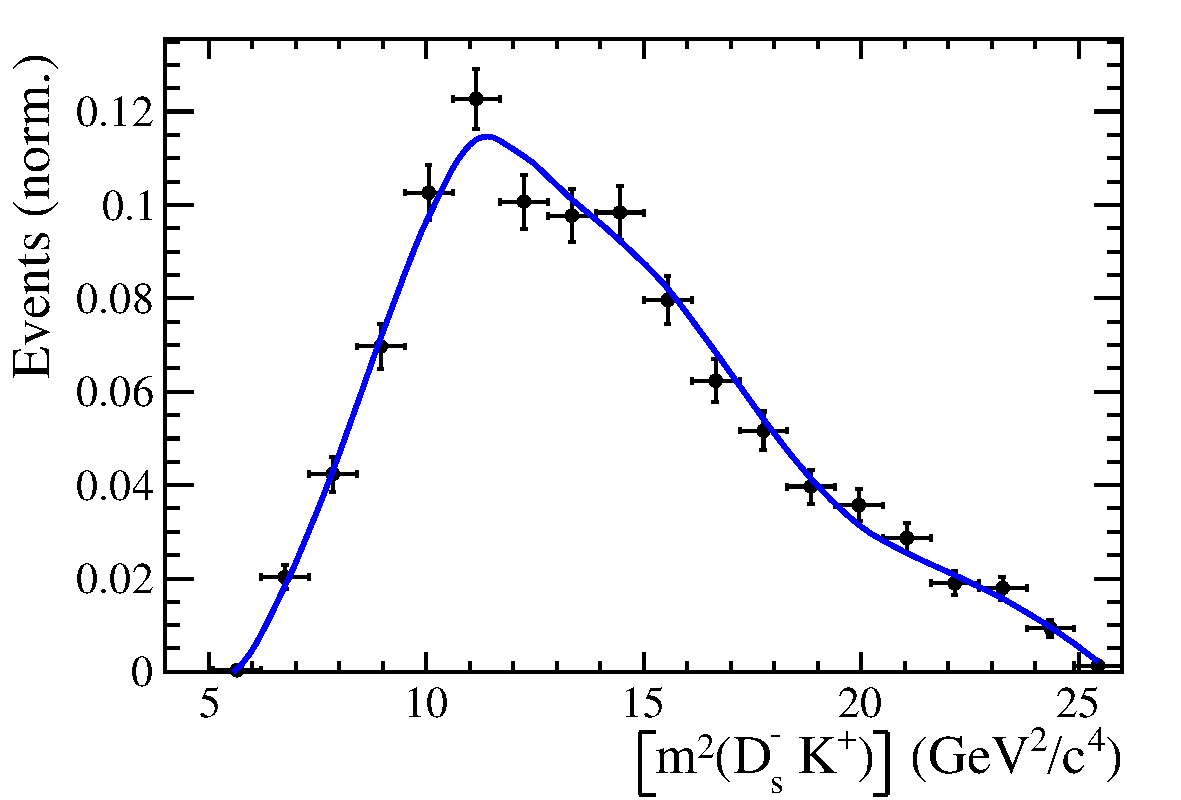
\includegraphics[width=0.45\textwidth, height = !]{figs/plots_toy/s_DsK-eps-converted-to.pdf} 
%		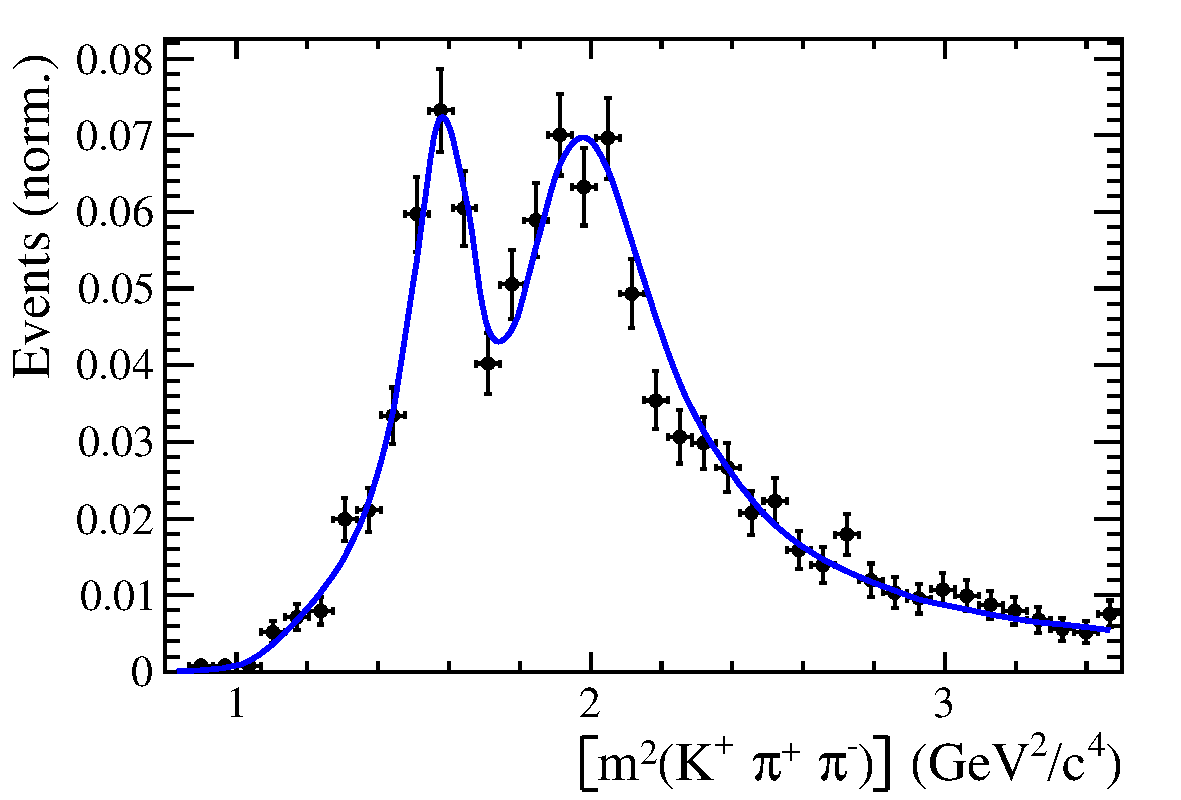
\includegraphics[width=0.45\textwidth, height = !]{figs/plots_toy/s_Kpipi-eps-converted-to.pdf}
%		 
%		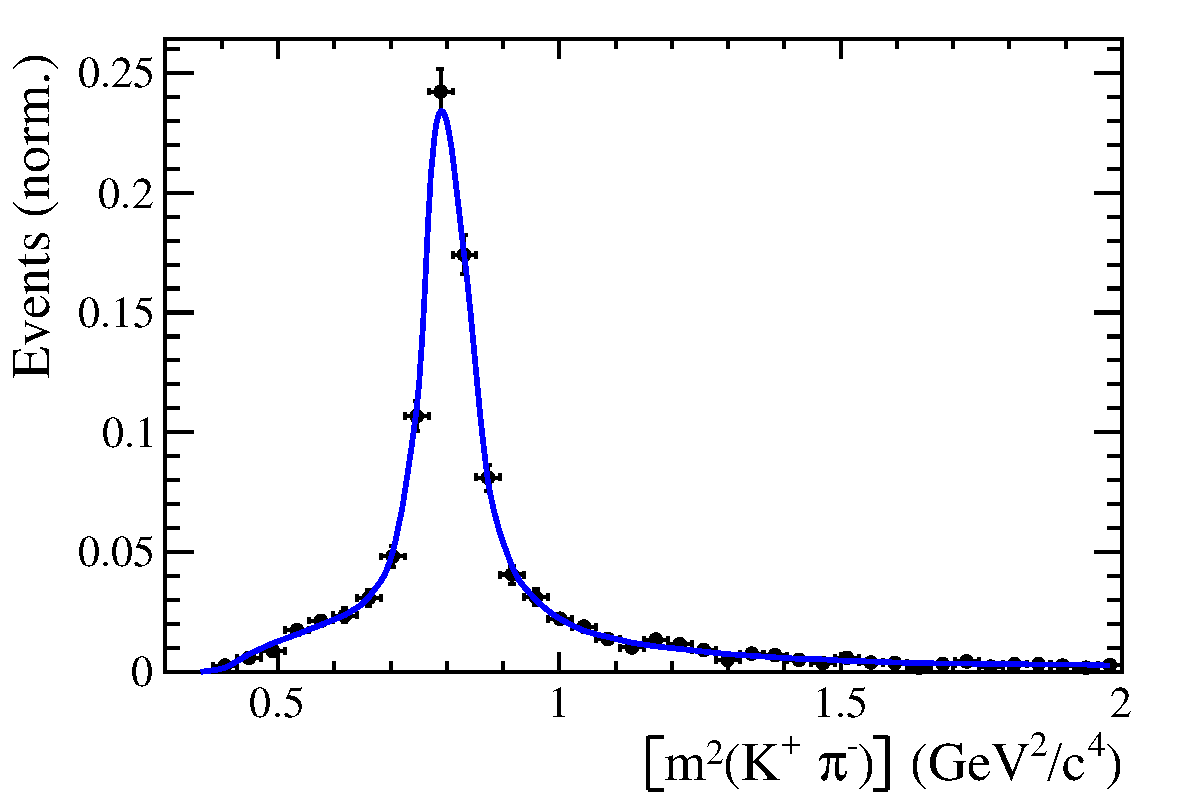
\includegraphics[width=0.45\textwidth, height = !]{figs/plots_toy/s_Kpi-eps-converted-to.pdf} 
%		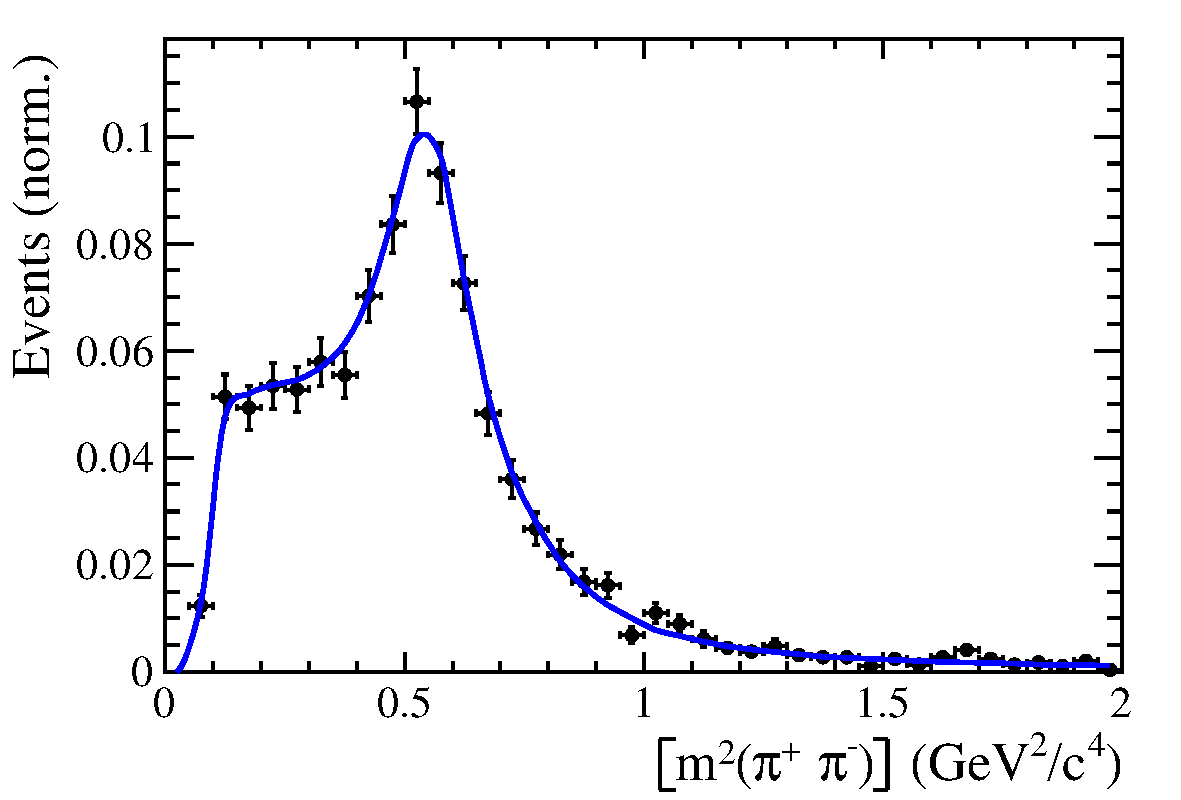
\includegraphics[width=0.45\textwidth, height = !]{figs/plots_toy/s_pipi-eps-converted-to.pdf}
%		
%		\caption{Example toy fit} 		
%	\end{figure}				
%
%
%	\begin{figure}[hp]
%	\centering
%		
%%		$D_s^+ K^- \pi \pi$      \hspace{2cm}     $D_s^- K^+ \pi \pi$   \hspace{2cm}   Combined
%%		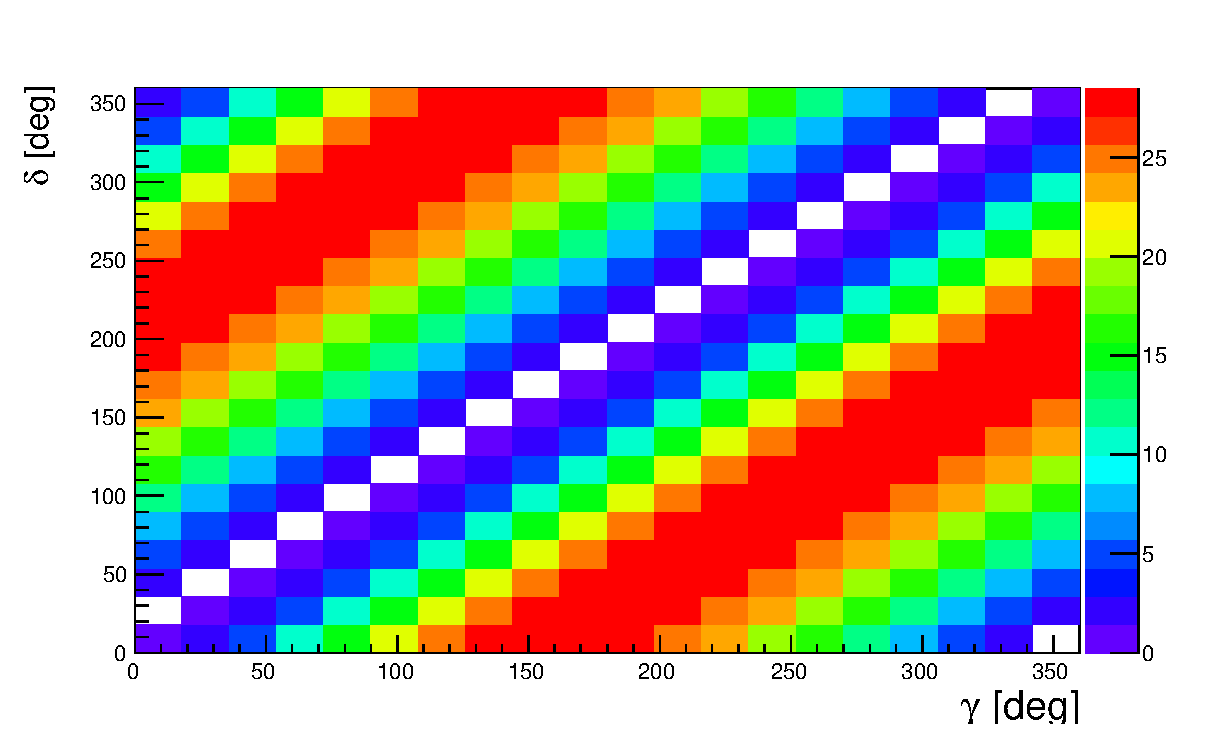
\includegraphics[width=0.4\textwidth, height = 4 cm{plots/LL_scan_m.eps} 
%%		\includegraphics[width=0.4\textwidth, height = 4 cm]{plots/LL_scan_p.eps} 
%		
%		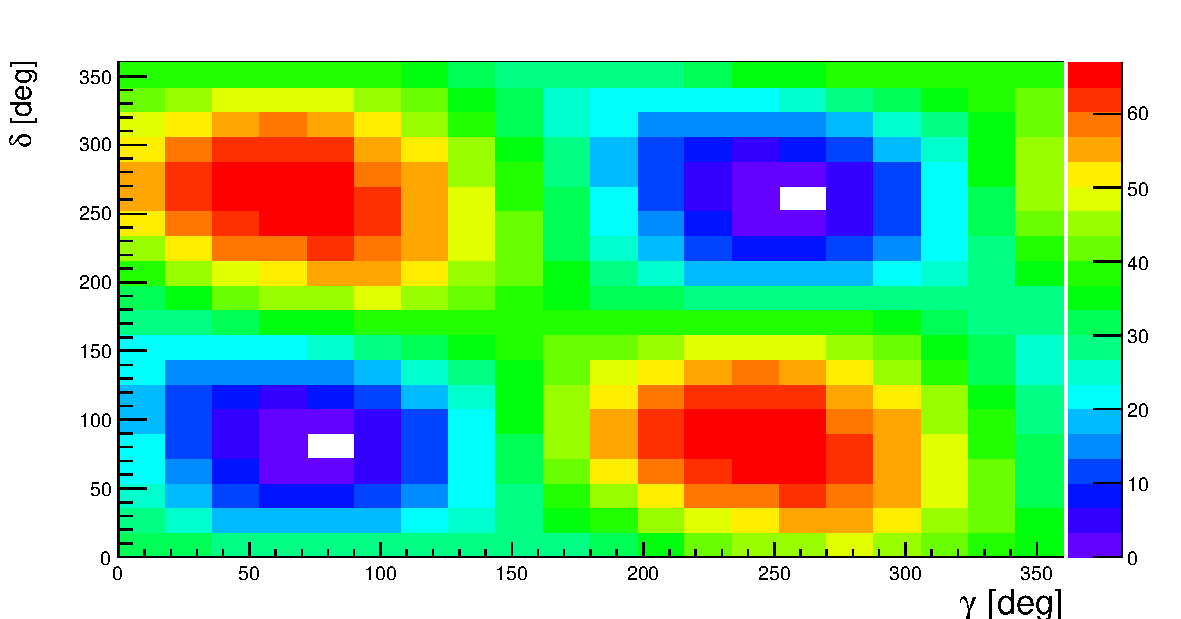
\includegraphics[width=0.45\textwidth, height = 4 cm]{plots/LL_scan-eps-converted-to.pdf} 
%		
%		Generated values: \\  $\gamma = 70^{\circ}, \delta = 100^{\circ}$ \\
%		Fit result:    \\ $\gamma = 74 \pm 15^{\circ}, \delta = 84 \pm 15^{\circ}$ \\
%		 ($\gamma = 254 \pm 15^{\circ}, \delta = 264 \pm 15^{\circ}$)
%
%		\caption{Likelihood scan} 		
%
%	\end{figure}	
%
%
%	\begin{figure}[hp]
%	\centering
%		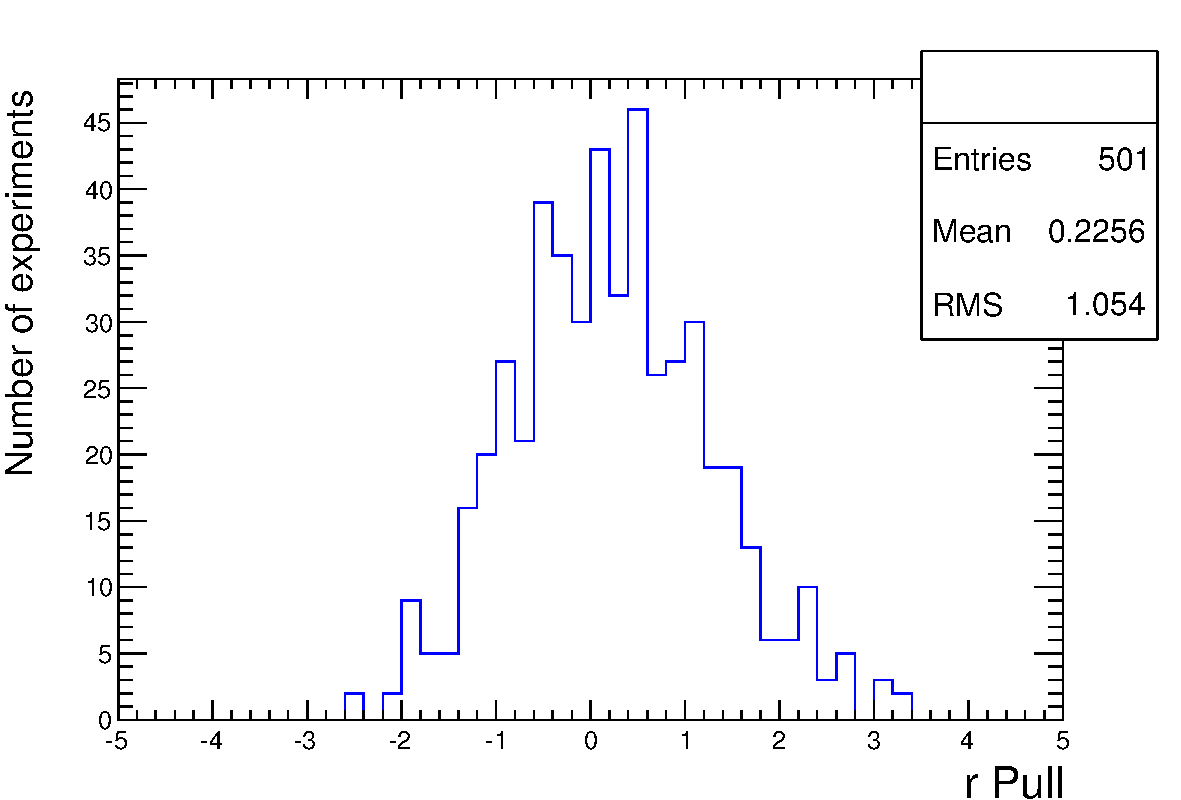
\includegraphics[width=0.4\textwidth, height = 3.cm]{figs/plots_toy/r_pull-eps-converted-to.pdf} 
%		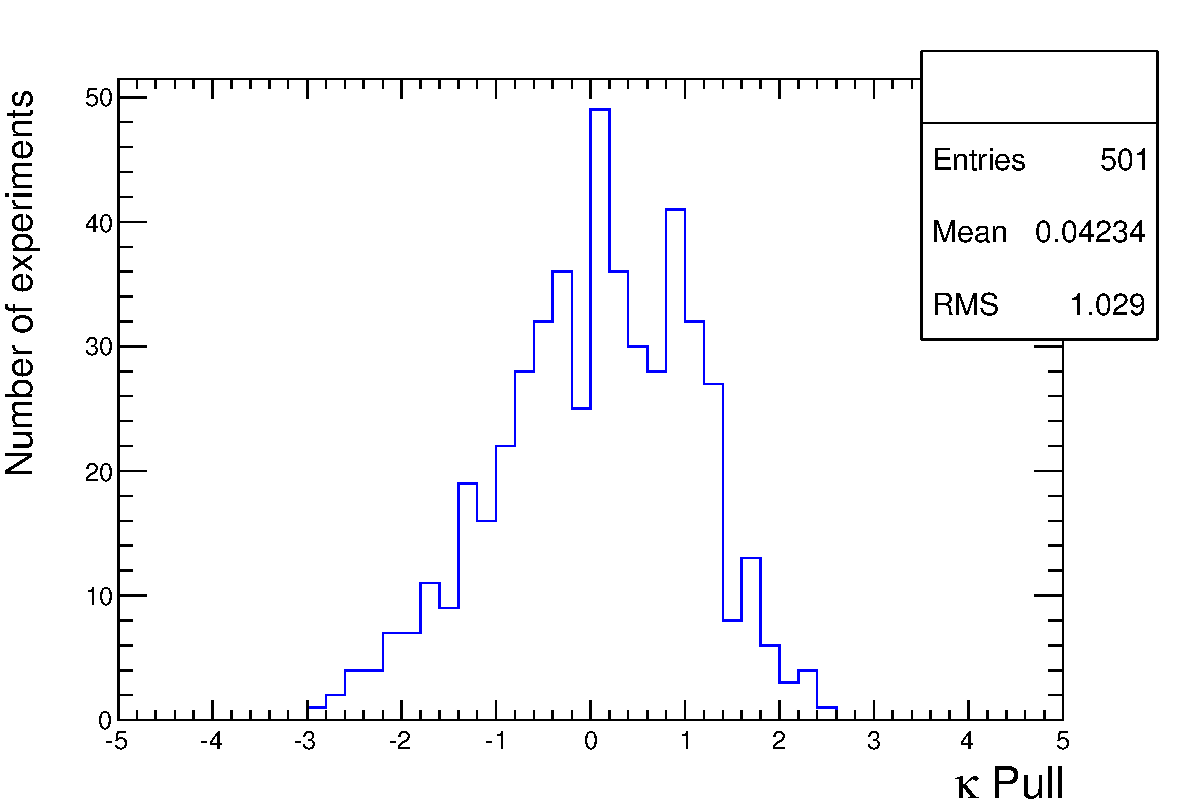
\includegraphics[width=0.4\textwidth, height = 3.cm]{figs/plots_toy/k_pull-eps-converted-to.pdf} 
%		
%		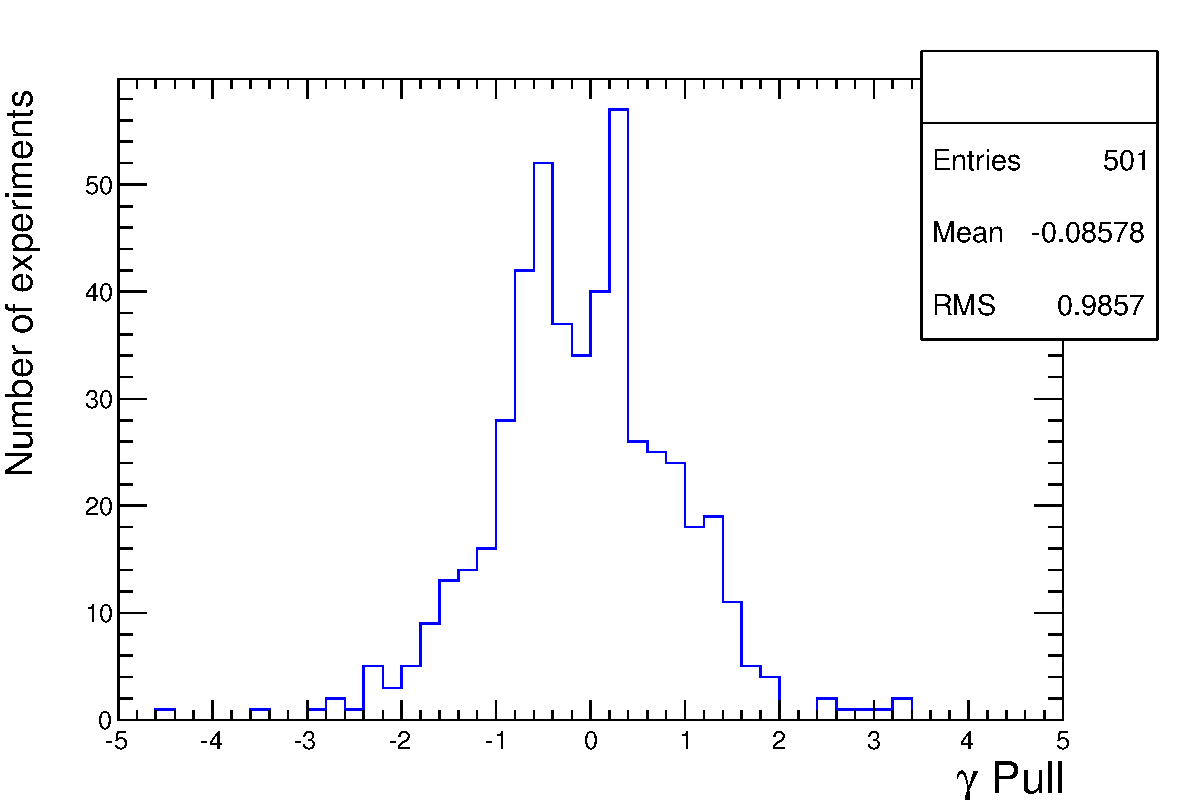
\includegraphics[width=0.4\textwidth, height = 3.cm]{figs/plots_toy/gamma_pull-eps-converted-to.pdf} 
%		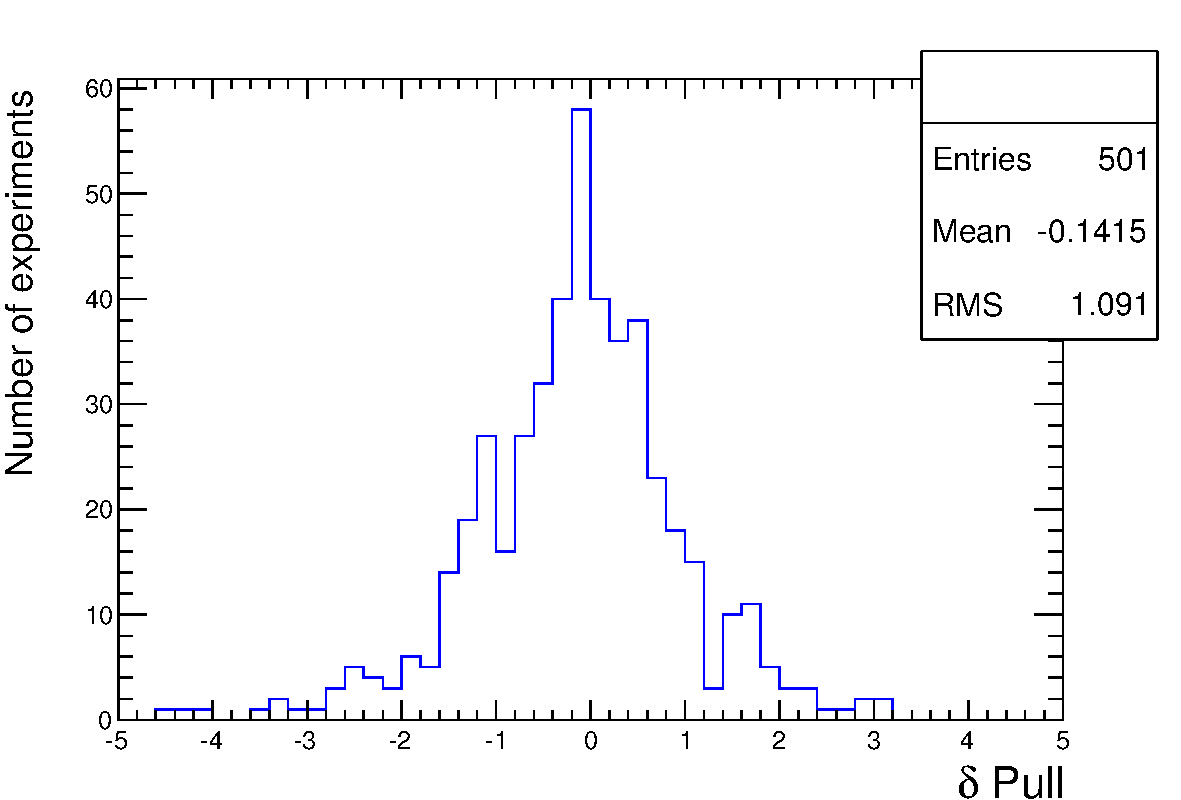
\includegraphics[width=0.4\textwidth, height = 3.cm]{figs/plots_toy/delta_pull-eps-converted-to.pdf} 
%
%		\caption{Pulls} 		
%
%	\end{figure}	
%	
%
%\clearpage	
%
%\begin{table}[h]
%	\caption{} 		
%  \scriptsize
%  \centering
%  \begin{tabular}
%    {l c c c c}
%    \hline \hline
%    & Generated &  Full PDF     &   Phasespace integrated  \\   \hline
%	$r$ & 0.4 & $0.38 \pm 0.06$   &  unstable \\
%	$\kappa$  & \textcolor{red}{0.2} & $0.23 \pm 0.13$ & 0.2 (fixed)  \\
%	$\delta$ & 100 & $99 \pm 22$ &  unstable\\
%	$\gamma$ & 70 & $70 \pm 17$  & unstable \\
%    \hline \hline
%  \end{tabular}
%
%  \begin{tabular}
%    {l c c c c}
%    \hline \hline
%    & Generated &  Full PDF    &   Phasespace integrated  \\   \hline
%	$r$ & 0.4 & $0.44 \pm 0.07$      & $0.43 \pm 0.11$  \\
%	$\kappa$  & \textcolor{red}{0.4} &$0.41 \pm 0.14$  & 0.4 (fixed)  \\
%	$\delta$ & 100 & $101 \pm 19$  & $95 \pm 41$ \\
%	$\gamma$ & 70 & $69 \pm 16$   & $66 \pm 40 $ \\
%    \hline \hline
%  \end{tabular}
%
%  \begin{tabular}
%    {l c c c c}
%    \hline \hline
%    & Generated &  Full PDF    &   Phasespace integrated  \\   \hline
%	$r$ & 0.4 & $0.41 \pm 0.08$     & $0.39 \pm 0.11$  \\
%	$\kappa$  & \textcolor{red}{0.6} & $0.60 \pm 0.13$  & 0.6 (fixed)  \\
%	$\delta$ & 100 & $98 \pm 17$ & $92 \pm 25$ \\
%	$\gamma$ & 70 & $68 \pm 17$ & $65 \pm 28$ \\
%    \hline \hline
%  \end{tabular}
%
%  \begin{tabular}
%    {l c c c c}
%    \hline \hline
%    & Generated &  Full PDF        &   Phasespace integrated  \\   \hline
%	$r$ & 0.4 & $0.42 \pm 0.09$    &  $0.39 \pm 0.09$ \\
%	$\kappa$  & \textcolor{red}{1.0} & $0.96 \pm 0.03$ &  1.0 (fixed)  \\
%	$\delta$ & 100 & $100 \pm 17$ &  $100 \pm 17$  \\
%	$\gamma$ & 70 & $66 \pm 17$ & $67 \pm 17$  \\
%    \hline \hline
%  \end{tabular}
%\end{table}
